% Options for packages loaded elsewhere
\PassOptionsToPackage{unicode}{hyperref}
\PassOptionsToPackage{hyphens}{url}
\PassOptionsToPackage{dvipsnames,svgnames,x11names}{xcolor}
%
\documentclass[
  12pt,
]{report}
\usepackage{amsmath,amssymb}
\usepackage{setspace}
\usepackage{iftex}
\ifPDFTeX
  \usepackage[T1]{fontenc}
  \usepackage[utf8]{inputenc}
  \usepackage{textcomp} % provide euro and other symbols
\else % if luatex or xetex
  \usepackage{unicode-math} % this also loads fontspec
  \defaultfontfeatures{Scale=MatchLowercase}
  \defaultfontfeatures[\rmfamily]{Ligatures=TeX,Scale=1}
\fi
\usepackage{lmodern}
\ifPDFTeX\else
  % xetex/luatex font selection
\fi
% Use upquote if available, for straight quotes in verbatim environments
\IfFileExists{upquote.sty}{\usepackage{upquote}}{}
\IfFileExists{microtype.sty}{% use microtype if available
  \usepackage[]{microtype}
  \UseMicrotypeSet[protrusion]{basicmath} % disable protrusion for tt fonts
}{}
\makeatletter
\@ifundefined{KOMAClassName}{% if non-KOMA class
  \IfFileExists{parskip.sty}{%
    \usepackage{parskip}
  }{% else
    \setlength{\parindent}{0pt}
    \setlength{\parskip}{6pt plus 2pt minus 1pt}}
}{% if KOMA class
  \KOMAoptions{parskip=half}}
\makeatother
\usepackage{xcolor}
\usepackage[margin=1in]{geometry}
\usepackage{graphicx}
\makeatletter
\def\maxwidth{\ifdim\Gin@nat@width>\linewidth\linewidth\else\Gin@nat@width\fi}
\def\maxheight{\ifdim\Gin@nat@height>\textheight\textheight\else\Gin@nat@height\fi}
\makeatother
% Scale images if necessary, so that they will not overflow the page
% margins by default, and it is still possible to overwrite the defaults
% using explicit options in \includegraphics[width, height, ...]{}
\setkeys{Gin}{width=\maxwidth,height=\maxheight,keepaspectratio}
% Set default figure placement to htbp
\makeatletter
\def\fps@figure{htbp}
\makeatother
\setlength{\emergencystretch}{3em} % prevent overfull lines
\providecommand{\tightlist}{%
  \setlength{\itemsep}{0pt}\setlength{\parskip}{0pt}}
\setcounter{secnumdepth}{-\maxdimen} % remove section numbering
\newlength{\cslhangindent}
\setlength{\cslhangindent}{1.5em}
\newlength{\csllabelwidth}
\setlength{\csllabelwidth}{3em}
\newlength{\cslentryspacingunit} % times entry-spacing
\setlength{\cslentryspacingunit}{\parskip}
\newenvironment{CSLReferences}[2] % #1 hanging-ident, #2 entry spacing
 {% don't indent paragraphs
  \setlength{\parindent}{0pt}
  % turn on hanging indent if param 1 is 1
  \ifodd #1
  \let\oldpar\par
  \def\par{\hangindent=\cslhangindent\oldpar}
  \fi
  % set entry spacing
  \setlength{\parskip}{#2\cslentryspacingunit}
 }%
 {}
\usepackage{calc}
\newcommand{\CSLBlock}[1]{#1\hfill\break}
\newcommand{\CSLLeftMargin}[1]{\parbox[t]{\csllabelwidth}{#1}}
\newcommand{\CSLRightInline}[1]{\parbox[t]{\linewidth - \csllabelwidth}{#1}\break}
\newcommand{\CSLIndent}[1]{\hspace{\cslhangindent}#1}
\usepackage{lineno}
\usepackage{amsmath}
\linenumbers
\usepackage{booktabs}
\usepackage{longtable}
\usepackage{array}
\usepackage{multirow}
\usepackage{wrapfig}
\usepackage{float}
\usepackage{colortbl}
\usepackage{pdflscape}
\usepackage{tabu}
\usepackage{threeparttable}
\usepackage{threeparttablex}
\usepackage[normalem]{ulem}
\usepackage{makecell}
\usepackage{xcolor}
\usepackage{multicol}
\usepackage{hhline}
\usepackage{hyperref}
\ifLuaTeX
  \usepackage{selnolig}  % disable illegal ligatures
\fi
\IfFileExists{bookmark.sty}{\usepackage{bookmark}}{\usepackage{hyperref}}
\IfFileExists{xurl.sty}{\usepackage{xurl}}{} % add URL line breaks if available
\urlstyle{same}
\hypersetup{
  pdftitle={Columbia Basin Research},
  pdfauthor={Markus Min},
  colorlinks=true,
  linkcolor={Maroon},
  filecolor={Maroon},
  citecolor={Blue},
  urlcolor={blue},
  pdfcreator={LaTeX via pandoc}}

\title{Columbia Basin Research}
\usepackage{etoolbox}
\makeatletter
\providecommand{\subtitle}[1]{% add subtitle to \maketitle
  \apptocmd{\@title}{\par {\large #1 \par}}{}{}
}
\makeatother
\subtitle{2023 Progress Report: A Bayesian multidirectional, multistate
model to resolve the migration pathways of adult Steelhead within the
Columbia River Basin}
\author{Markus Min}
\date{12 December 2023}

\begin{document}
\maketitle

{
\hypersetup{linkcolor=}
\setcounter{tocdepth}{2}
\tableofcontents
}
\setstretch{1.1}
\hypertarget{executive-summary}{%
\chapter{Executive summary}\label{executive-summary}}

Columbia River Steelhead, who spend more time as adults in freshwater
than any other salmonid in the basin, have notoriously complex adult
migration pathways, characterized frequently by indirect pathways home,
overshooting natal tributaries, and falling back over and through
hydroelectric dams. Previous studies have characterized specific
movements of interest (i.e., overshoot and fallback) and examined the
effect of some factors on these movements, but have not presented a
comprehensive view of the adult Steelhead migration.

Here, we present a progress update on a new modeling framework that is
capable of modeling the entire adult migration of Steelhead, including
upstream movements, downstream movements, and movements into
tributaries. This modeling framework translates the Columbia River Basin
into a series of interconnected states, each representing a reach of the
mainstem Columbia or Snake River between hydroelectric dams or a
tributary that flows into them. We converted detections of over 60,000
Steelhead over 17 years from each of the hundreds of PIT tag detection
sites in the Columbia River Basin into a sequence of state visits for
each fish, and fit a Bayesian multistate model to these data using the
Stan programming language. This model also uses the network of PIT tag
antennas in each tributary to correct for detection efficiency in each
of these tributaries.

Work on this model is ongoing. A previous progress update on this model
presented results for a model without any covariates
(\textbf{Min2022?}). At this time, the model code has been written and
is set up to run with key covariates included (rear type, origin, spill,
temperature, and year), but final results are not yet available due to
the long run time of the model (on the order of weeks) and the
difficulty of securing the computational resources required to run this
model. Final model results should be available in early 2024.

\hypertarget{introduction}{%
\chapter{Introduction}\label{introduction}}

Steelhead (anadromous \emph{Oncorhynchus mykiss}) in the Columbia River
Basin, including all those found above Bonneville Dam, are listed under
the Endangered Species Act. The five Columbia River Basin distinct
population segments (DPSs) were first listed in the late 1990s, and are
all currently listed as threatened. Despite their protected status and
continued recovery efforts, counts of returning Steelhead to Bonneville
Dam have been lower in the last five years than they were at the time of
listing, and recently completed 5-year reviews for Columbia River
Steelhead reaffirmed their status as threatened (NMFS 2022a, 2022b,
2022c, 2022d).

One element of the life history of Columbia River Basin Steelhead that
may make them more vulnerable to anthropogenic modifications of the
Columbia River is their adult migration. Relative to other salmonids,
Steelhead from the Columbia River Basin spend longer in freshwater as
adults. Essentially all populations of Steelhead in the Columbia River
Basin are stream-maturing (Busby \emph{et al.} 1996), meaning that these
fish enter freshwater in a sexually immature state and then spend up to
a year in freshwater prior to spawning. Also known as summer Steelhead,
these fish enter freshwater between May and October and spawn the
following spring, typically between March and May (Busby \emph{et al.}
1996). Between their entry into freshwater and arrival at spawning
grounds, Columbia River Steelhead exhibit considerable variability in
their migration patterns. Virtually all interior Columbia River
Steelhead overwinter in freshwater; the majority of individuals are
known to overwinter in tributaries, but up to 20\% of individuals in a
given year have been observed to overwinter in the hydrosystem, which
comprises the mainstem habitat between the hydroelectric dams in the
federal Columbia River power system (Keefer \emph{et al.} 2008).
Additionally, as individuals migrate upstream toward natal tributaries,
the majority of individuals have been observed to temporarily stage in
nonnatal tributaries downstream of their natal tributary (High \emph{et
al.} 2006). This behavior increases with increasing mainstem river
temperature, indicating the use of these colder waters as coldwater
refugia (High \emph{et al.} 2006). These highly variable movement
patterns and increased duration in freshwater make Steelhead more
vulnerable to the hazards faced in freshwater.

Descending dams, also known as fallback (Boggs \emph{et al.} 2004), is
another common behavior observed in adult Steelhead, with about 20\% of
Steelhead observed to fall back over at at least one mainstem dam (Boggs
\emph{et al.} 2004). This behavior can occur as individuals are
migrating upstream to natal tributaries, which we refer to as ``en-route
fallback'', but can also occur once individuals have ascended mainstem
dams upstream of natal tributaries (a behavior known as overshoot). We
refer to fallback that has occurred after Steelhead have overshot natal
tributaries as ``post-overshoot fallback'', and in this case fallback is
necessary for individuals to return to natal tributaries. Overshoot and
fallback can affect the ability of individuals to successfully home to
spawning grounds, and therefore are consequential for the persistence of
ESA-listed populations. Individuals that fall back during their upstream
migration (prior to reaching or overshooting their natal tributary) are
less likely to return to their natal tributaries or hatcheries (Bjornn
\emph{et al.} 2000; Keefer \emph{et al.} 2005). Furthermore, migration
success to natal tributaries decreases with increased overshooting
(Richins and Skalski 2018), and many overshooting fish are observed to
stray to tributaries upstream of the overshoot dam.

The decreased migration success associated with overshoot and fallback
may be due to the hazardous nature of downstream passage for adults,
which is often limited to the powerhouse during the primary months that
Steelhead are overwintering (Khan \emph{et al.} 2013). The incidence of
mortality for adult Steelhead passing downstream at dams is highly
variable, but recent estimates of 48-hour survival at McNary Dam
indicate around 90\% survival for individuals passing through turbines
and 97\% survival for individuals passing through the spillway
(Normandeau Associates 2014). Mortality in downstream passage routes is
implicated by low survival of Steelhead kelts, which decrease with
increasing number of dams that must be navigated as they move downstream
to the ocean, with mortality of 84-96\% for kelts released at Lower
Granite Dam, 38-40\% at McNary Dam, and 20-37\% at John Day Dam
(Wertheimer and Evans 2005).

Because of the association between overshoot and fallback and decreased
migration success, previous studies have investigated the influence of
various factors on the incidence of these behaviors. Rates of overshoot
have been observed to vary considerably among populations, with some
studies finding a positive relationship with increasing mainstem water
temperature and hatchery rearing upstream of the natal tributary
(Richins and Skalski 2018). In spring-summer Chinook, Boggs \emph{et
al.} (2004) observed a positive relationship between fallback rates and
river discharge. However, these previous studies have looked at these
various factors only in isolation and for specific movements, which
complicates the modeling of emergent properties and interactions between
behaviors, environmental conditions, and populations, and can be
challenging in the face of sparse data in some settings. In this
progress report, we present a multistate model that is capable of
modeling the entire adult Steelhead migration, from first detection at
Bonneville Dam to arrival in natal tributaries. This model, which does
not constrain movement to only be upstream, allows the complex,
multidirectional movement of adult Steelhead to be modeled in full and
allows many movements of interest, including fallback, overshoot, and
homing, to be estimated in a single framework. The data used in this
model were passive integrated transponder (PIT) tag detection histories.
This modeling framework is capable of accommodating the effect of
multiple categorical and continuous covariates on movement probabilities
at each step within the migration. By examining how Steelhead movement
probabilities, particularly those of conservation concern, such as
overshoot, fallback, homing, and straying, vary by population and are
influenced by various factors, this modeling framework will improve our
understanding of how both environmental and anthropogenically influenced
conditions affect how Steelhead move within the Columbia River and its
tributaries.

\hypertarget{methods}{%
\chapter{Methods}\label{methods}}

\hypertarget{study-area}{%
\section{Study area}\label{study-area}}

\begin{figure}
\centering
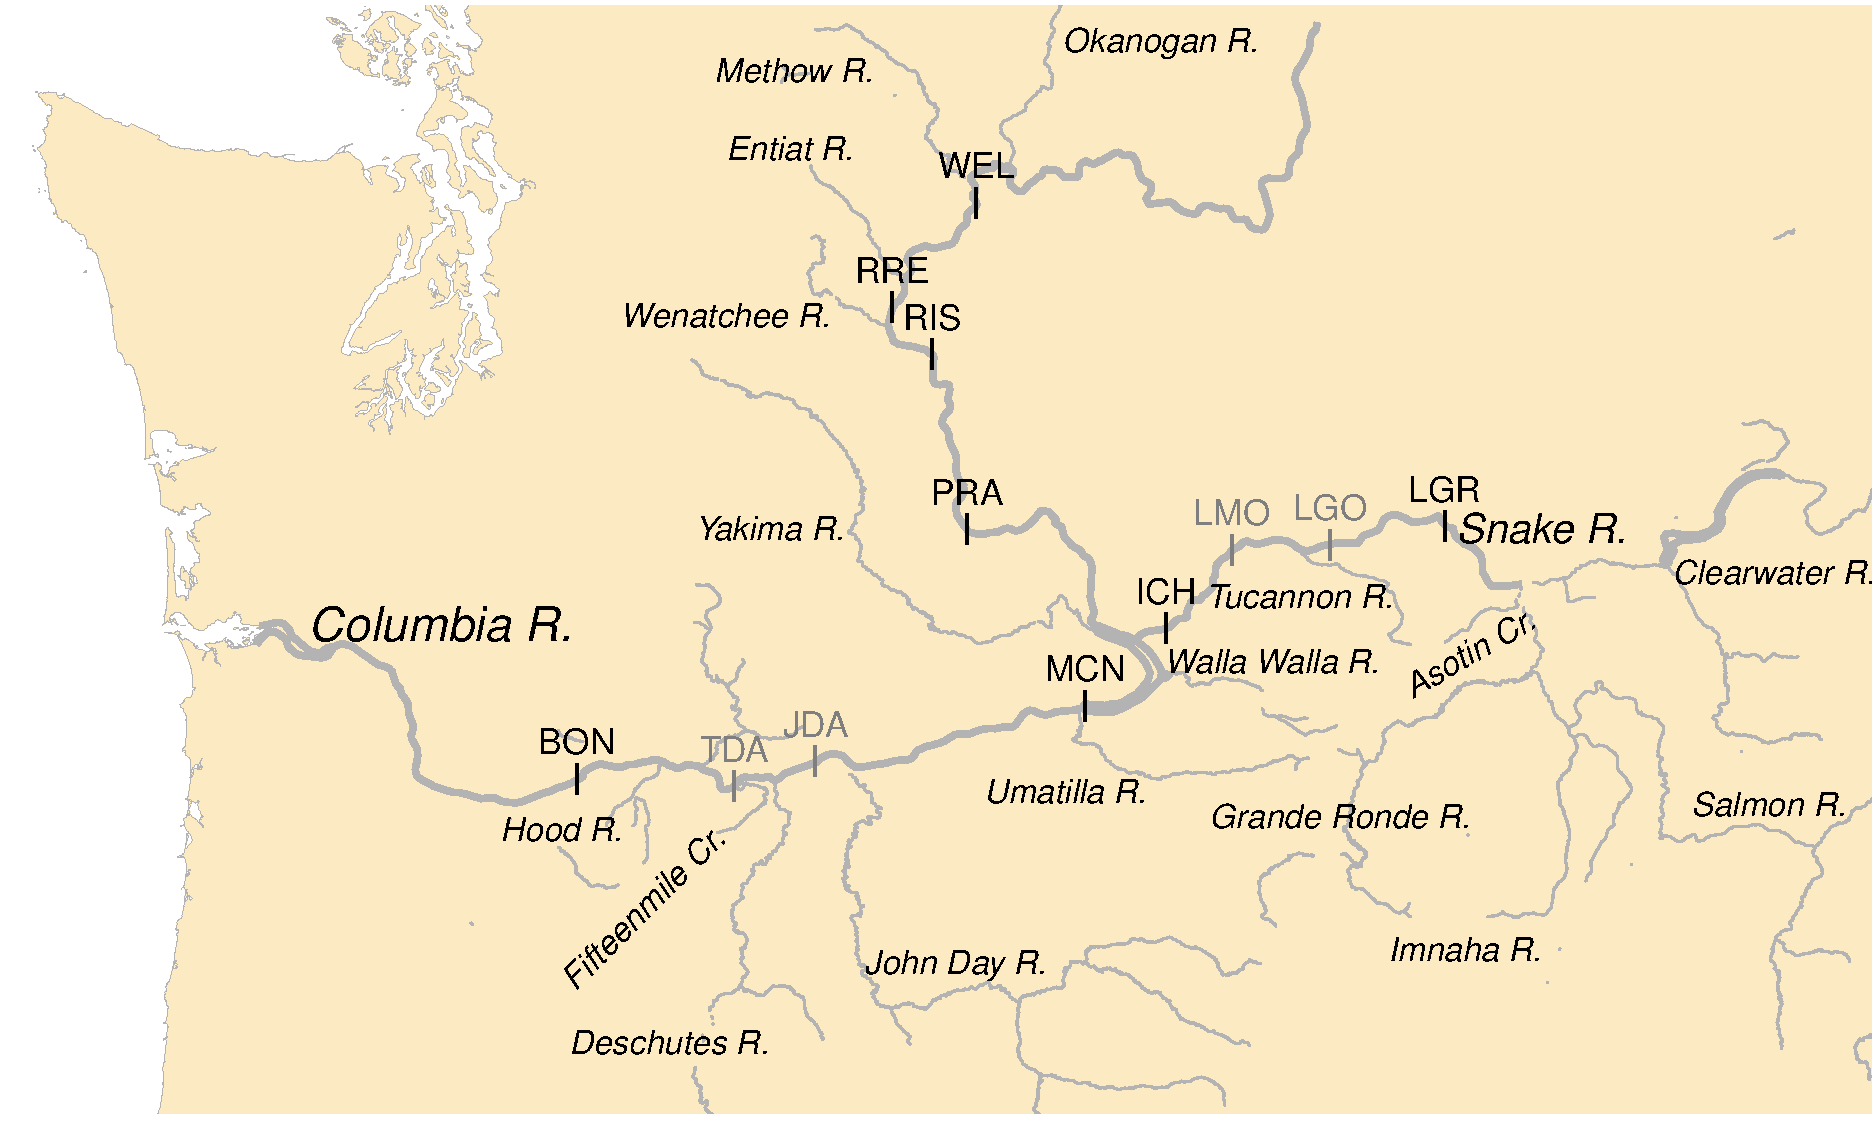
\includegraphics[width=1\textwidth,height=\textheight]{.//figures/CRB_map_pres_dams.pdf}
\caption{Figure 1. The study area, showing all mainstem dams that
currently have PIT arrays. Dams that are used to delineate states in the
model are in black, whereas those that are not are in grey. Tributaries
where fish in our dataset originated are labeled. BON = Bonneville Dam;
TDA = The Dalles Dam; JDA = John Day Dam; MCN = McNary Dam; PRA = Priest
Rapids Dam; RIS = Rock Island Dam; RRE = Rocky Reach Dam; WEL = Wells
Dam; ICH = Ice Harbor Dam; LMO = Lower Monumental Dam; LGO = Little
Goose Dam; LGR = Lower Granite Dam.}
\end{figure}

\hypertarget{modeling-overview}{%
\section{Modeling overview}\label{modeling-overview}}

\begin{figure}
\centering
\includegraphics[width=1\textwidth,height=\textheight]{.//figures/full_model_diagram.jpg}
\caption{Figure 2. The model schematic. There were 29 states in our
model: 9 mainstem states (outlined in blue), 19 tributary states
(outlined in green), and the absorbing ``loss'' state (not pictured).}
\end{figure}

In our model, the Columbia River and its tributaries are modeled as a
series of connected states, with states defined as either reaches of the
mainstem Columbia or Snake River between dams with PIT tag detection
capabilities in the adult ladders or tributaries with PIT tag detectors.
Fig. 2 shows all of the states in our model; movements over some dams
(e.g., The Dalles Dam, John Day Dam, Lower Monumental Dam, or Lower
Goose Dam) were not explicitly modeled due to these dams not having PIT
tag detection capabilities for the duration of our study period.

An additional state in our model not shown in the schematic, but which
can be reached from any state, is the absorbing ``loss'' state, which a
fish enters once the detection history ends. Once a fish has entered the
loss state, it can no longer leave it. Movements into the loss state are
either mortality (via natural mortality, harvest, mortality due to the
hydrosystem, etc.), the start of kelt movement following spawning (as
all kelt movements were removed to isolated the adult migration prior to
spawning), or unobserved movements out of the state, which could be due
to missed detections at PIT tag antennas, movements into areas without
PIT tag detectors (e.g., certain tributaries), or movements into
tributaries that failed to reach PIT tag antennas.

\hypertarget{preparing-data}{%
\section{Preparing data}\label{preparing-data}}

\hypertarget{accessing-pit-tag-data}{%
\subsection{Accessing PIT tag data}\label{accessing-pit-tag-data}}

PIT tag data were obtained from the Columbia Basin PIT Tag Information
System (PTAGIS). Only known-origin individuals (based on known release
sites) were included in this dataset. To ensure that only individuals
marked as juveniles were retained in the dataset, all individuals that
were greater than 350 mm at time of marking were removed. To select
returning adults, only individuals that were seen in the adult fishways
at Bonneville Dam were selected. To ensure that there were enough data
for each population included in this dataset, only populations (defined
as the combination of natal tributary and rear type) that had at least
350 individuals distributed across 8 run years were retained.
Additionally, only populations with instream PIT tag detections sites in
their natal tributaries were retained; if sufficient instream detection
sites only became available during the later part of our study period,
only individuals from those years were retained. Run years were
separated by June 1 of each year, and run year 2005/2006 (beginning on
June 1, 2005) was selected as the first year in our dataset. In total,
populations from 17 natal tributaries met these criteria: 11 tributaries
of the Columbia (Deschutes River, John Day River, Hood River,
Fifteenmile Creek, Umatilla River, Yakima River, Walla Walla River,
Wenatchee River, Entiat River, Okanogan River, and Methow River) and six
tributaries of the Snake (Tucannon River, Asotin Creek, Clearwater
River, Salmon River, Grande Ronde River, and Imnaha River). Once the tag
codes were identified for each of these tributary populations, a
complete tag history report was run in PTAGIS for all of the tag codes
in our dataset.

\hypertarget{processing-pit-tag-data-into-detections-at-various-sites}{%
\subsection{Processing PIT tag data into detections at various
sites}\label{processing-pit-tag-data-into-detections-at-various-sites}}

To convert detections of fish at individual PIT tag antennas into a
history of movements between different reaches of the Columbia, Snake,
and their tributaries, it was first necessary to interpret detections at
different PIT tag antennas. For instream tributary detection sites, as
well as mainstem sites in between dams, processing only entailed
assigning detections at these sites to the corresponding model state.
For detection sites at dams, more involved processing was required to
interpret detections.

The first step in interpreting detections at dams was to identify the
multiple passage routes associated with each dam. In many cases,
multiple passage routes were grouped together into a single
interrogation site, and assigning antennas to these different passage
routes was necessary to interpret how fish were utilizing these passage
routes. For example, antennas at Ice Harbor Dam are all grouped together
in PTAGIS as ``Ice Harbor Dam (combined)'', when these antennas are
actually in three different passage routes: the North Shore Ladder, the
South Shore Ladder, and the Juvenile Bypass System.

The second step was to identify, when possible, entrance and exit
antennas within each upstream passage route. By distinguishing entrance
and exit antennas, we were able to identify when fish detections in
adult fishways were not ascents, but were rather aborted ascent attempts
or descents. Entrance and exit antennas were only distinguished when
either two distinct groupings of antennas existed in separate parts of
the same passage route, or in the case of Bonneville Dam, when there are
enough consecutive weirs with PIT tag detection antennas to separate the
antennas in these weirs into entrance and exit antennas. When fish were
only seen at entrance antennas, this was noted to be an aborted
ascension attempt. When fish were first seen at the exit antennas at an
adult fish ladder and last seen at the entrance antennas of the same
fish ladder, this was noted to be a descent through the ladder. If a
fish was first seen at the entrance antennas and last seen at the exit
antennas, this was noted to be an ascent. Entrance and exit antennas
were identified at all adult fishways except for McNary Dam Washington
Shore Ladder (prior to March 2006), Priest Rapids Dam, Rock Island Dam,
Rocky Reach Dam, Wells Dam (prior to 2013), and Ice Harbor Dam.

Additionally, we identified antennas in adult fish facilities/traps at
ladders. For most dams (e.g., Ice Harbor Dam, Priest Rapids Dam, or
Lower Granite Dam, where traps were operated but adults were returned
after processing), we treated detections in the adult fish facility the
same as detections in other parts of the adult ladder, as adults were
not removed. However, in the case of Wells Dam, trapped fish were either
moved to the hatchery or trucked off-site. As such, any terminal
detections in the trap at Wells Dam were classified as terminal trapping
events, and were classified as fish moving to the absorbing ``loss''
state.

Once the antennas had been appropriately assigned, a 48-hour threshold
was used to distinguish separate detection events at a site. However, in
some passage routes fish were observed in the same route for days at a
time, so no time threshold was set, and instead we used the sequence of
antennas to distinguish separate detection events at a site. For
example, some individual fish did not exit the Washington shore passage
route at Bonneville Dam for upwards of 100 days, so new visits to this
site were only distinguished by new visits to the entrance antennas,
regardless of the amount of time between detections at other antennas in
the passage route.

\hypertarget{turning-detections-at-different-sites-into-state-transitions}{%
\subsection{Turning detections at different sites into state
transitions}\label{turning-detections-at-different-sites-into-state-transitions}}

With antennas appropriately assigned to different passage routes and the
sequence of antenna detections at the adult fishways used to interpret
directionality, the output from the previous script was used as input
into the next script, which converted a history of detections at sites
into a history of movements between states, as defined in Fig. 2. For
detections at sites in the fish passage routes at dams, the
directionality of movement, as assigned in the previous script, was used
to inform transitions between states. Ascents at dams indicated a
transition from the downstream state to the upstream state; descents at
dams (either through the juvenile bypass system or descents through the
ladder) indicated a transition from the upstream state to the downstream
state. Aborted ascension attempts were noted, but interpreted as no
transition from the current state. Detections in tributary sites that
immediately followed detections in mainstem sites were interpreted as
transitions from the mainstem state into the tributary. Once a fish
transitioned into a given state, any subsequent detections in that state
were ignored, as they did represent transitions between states.
Therefore, if fish were detected at sites within the same tributary
consecutively, or if fish were detected at instream sites in the
mainstem following transition into that mainstem state, these detections
were ignored.

With the exception of a few downstream routes, such as the spillway at
Lower Granite Dam following the installation of the PIT tag antennas in
2020, or the Bonneville Corner Collector, PIT tag detection capabilities
at each dam were limited to the adult fish ladders and the juvenile
bypass system. As such, PIT tag antennas have historically been unable
to directly monitor fallback at dams, unless an individual subsequently
reascends the dam (Boggs \emph{et al.} 2004). With the installation of
instream antennas in natal tributaries, fallback to home has been
monitored (Richins and Skalski 2018) by noting when individuals entered
natal tributaries downstream of a dam that was previously ascended. In
this study, we monitored fallback to the greatest extent possible with
the current configuration of PIT tag antennas by using our knowledge of
the connections between states in our model to note when downstream
movements must have occurred. For example, if we noted two consecutive
ascents at Bonneville Dam, or if we observed a fish in the John Day
River after ascending McNary Dam, we added a fallback event in between
these events. In this way, we included fallback that occurred on the
mainstem downstream of the natal tributary (similar to Boggs \emph{et
al.} (2004)), fallback to home (similar to Richins and Skalski (2018)),
and other fallback movements, such as fallback upstream of the natal
tributary that did not end in homing. Using a similar strategy of
interpolating state transitions based on state connectivity, we also
interpolated upstream movements that were missed by the PIT tag antennas
in adult fish ladders, although these missed detections were very
infrequent, as detection probabilities in adult ladders is close to
100\% (Richins 2017).

Once we determined a history of movement between states, we then subset
this movement history to eliminate any movement that occurred as a
juvenile or as a kelt in order to isolate only the portion of the adult
migration prior to reaching spawning areas. Based on manual inspection
of detection histories, juvenile movements were identified using the
following criteria: (1) any detections within 90 days of juvenile
release; (2) any detections on or before June 15 of the same year that
an individual was released, or detections on or before June 15 in a
given year if individual was released on or after July 1 of the previous
year. The June 15 cutoff date was chosen based on the timing of juvenile
outmigration at Bonneville Dam, 95\% of which occurs before this date in
nearly every run year (data from CBR DART). Kelt movement was identified
as any downstream movement occurring between March and July (following
spawning). Repeat spawners were also identified in the dataset based on
detections at the Bonneville Dam adult ladders occurring at least 180
days after they were initially seen at Bonneville Dam. For the purposes
of our analysis, repeat spawners were treated as new fish when they
returned to Bonneville Dam.

\hypertarget{model-covariates}{%
\section{Model covariates}\label{model-covariates}}

\hypertarget{temperature-data}{%
\subsection{Temperature data}\label{temperature-data}}

Temperature was included as a covariate for certain fish movements.
Daily average forebay and tailrace temperatures were queried from the
Columbia Basin Conditions portal from the DART page for the eight dams
for which movement was explicitly modeled (BON, MCN, PRA, RIS, RRE, WEL,
ICH, and LGR). Due to the noise and gaps inherent to the temperature
data, a series of steps were performed to clean this data. To address
outliers in the temperature data, two steps were taken. First, plots of
temperature were manually inspected and sequential runs of temperature
points that were outside of the range of possible values for that time
of year were removed. Next, a filtering algorithm was applied to remove
any temperature values that were more than four degrees outside of the
interannual average temperature value for that day of the year, as well
as any values that were more than two degrees outside of the 7-day
moving average. To address the incomplete temporal resolution for
temperature at each dam in our modeling framework, a state-space model
was fit using the MARSS package (\textbf{Holmes2012?}). This model took
as inputs the cleaned temperature data at the forebay and tailrace for
the eight dams (a total of 16 temperature time series). The model was
structured with only a single process (the basin-scale temperature) and
16 observations of that process. Each dam had a different offset/bias
term (8 total). Model-estimated temperatures on each day for each dam
were then exported by using the estimate of the basin-scale temperature
plus the dam-specific offset.

To estimate the temperatures experienced by fish, the median residence
time in each state in our model was first calculated. This was done by
calculating the amount of time spent in each state by each fish in our
dataset (the difference between date on which a fish was observed
exiting a state and the date on which a fish was observed entering a
state) and then taking the median time spent in each state across all
fish. To estimate the mean temperature experienced by the fish while in
a state, the mean temperature across a window of time (defined as the
date a fish was observed entering a state plus the median residence time
for all fish in that state) was taken. The downstream dam for a state
was used as the source of temperature data for that state.

\hypertarget{spill-data}{%
\subsection{Spill data}\label{spill-data}}

Daily average spill (in thousands of cubic feet per second) were queried
from the Columbia Basin Conditions portal from the DART page for the
eight dams for which movement was explicitly modeled (BON, MCN, PRA,
RIS, RRE, WEL, ICH, and LGR). Spill data was processed in two different
ways to facilitate the inclusion of two hypothesized relationships
between spill and fish fallback over dams. Fallback over dams can be
divided into two distinct types of fallback: en-route fallback, which
occurs when fish fall back prior to reaching their natal tributaries,
and post-overshoot fallback, which occurs when fish fall back after
overshooting natal tributaries (having ascended the dam directly
upstream of their natal tributary).

En-route fallback goes against the desired direction of movement for all
fish, as their goal is to continue traveling upstream. Our hypothesis
surrounding en-route fallback is that it is involuntary; i.e., that it
occurs as a result of river conditions (spill, flow) and/or individual
condition. As such, our hypothesis for the relationship between spill
and en-route fallback is that it is related to the volume of spill, as
this would serve to push fish back downstream over a dam via the
spillway (or alternatively, serves as a proxy for flow conditions in the
river). The approach that we used for this spill covariate is the same
as was used for temperature, i.e., the use of windows and taking the
average spill during that window.

In contrast, post-overshoot fallback is a desirable outcome for all
fish, as this movement helps them get closer to their natal tributary.
Our hypothesis surrounding post-overshoot fallback is that it is
voluntary; i.e., that it occurs when fish make the decision to want to
go back downstream and towards their natal tributaries. As such, our
hypothesis for the relationship between spill and post-overshoot
fallback is that it is related to the presence of spill, as the presence
of spill allows fish to find a safe route back downstream. This is based
in large part on the work of Richins \& Skalski (2018) and Wertheimer
(2007), who found that even small amounts of surface flow were effective
for routing steelhead kelts away from turbines, indicating that the
availability of surface passage options may be more important than the
volume of flow. The approach we used for this covariate was to find the
total number of days with any amount of spill in the months of January,
February, and March, which is when post-overshoot fallback is predicted
to occur (after overwintering).

\hypertarget{statistical-methods}{%
\section{Statistical methods}\label{statistical-methods}}

\hypertarget{modeling-detection-efficiency-in-tributaries}{%
\subsection{Modeling detection efficiency in
tributaries}\label{modeling-detection-efficiency-in-tributaries}}

Over the course of our study period, the network of PIT tag detection
arrays in tributaries was highly dynamic, as antennas were installed,
decommissioned, and upgraded. From 2010 to 2018, the number of tag
detection arrays in tributaries almost tripled (Morrisett 2018), and in
some years of our study, the tributaries in our model had no active
antennas at all (Richins 2017). As a consequence, our ability to detect
fish entering these tributaries varied considerably both temporally and
spatially (between tributaries).

To address this, we estimated detection efficiency in tributaries by
calculating the detection efficiency at the PIT tag detection site
closest to the river mouth (i.e., the confluence of the tributary with
either the Columbia or Snake River). We estimated detection efficiency
by taking the individuals that were seen at detection sites upstream of
the river mouth site and calculating what proportion were seen at the
river mouth site. For 14 of the 17 tributaries in our model (Table 1),
we identified a PIT tag detection site on the mainstem tributary
suitable for calculating detection efficiency; three tributaries (the
Clearwater River, Salmon River, and Grande Ronde River) lacked a
suitable site and therefore detection efficiency was not calculated for
these tributaries.

In our estimation of detection efficiency, we included two covariates:
(1) a categorical covariate representing different antenna
configurations, and (2) a covariate for the effect of discharge.
Different categorical covariates were chosen based on the operational
history of each interrogation site. We identified major changes in site
configuration which were likely to have affected the detection
efficiency at these sites, such as the installation of new antennas,
arrays being moved, or components being upgraded. The years in which
these changes occurred were then used to inform which categorical
covariate for antenna configuration was used. We chose to include
discharge as a covariate for detection efficiency as well because of the
relationship between discharge and river stage, which affects the volume
of the river covered by the range of the antennas (see Fig. 3 for an
example). Discharge data were queried from USGS by finding the station
on the interactive USGS dashboard
(\url{https://dashboard.waterdata.usgs.gov}) closest the river mouth
array and navigating to the data page for the specific site. Discharge
data were available for all tributaries except Fifteenmile Creek and the
Imnaha River; these tributaries therefore had detection efficiency
estimated only via the categorical covariate (intercept) for antenna
configuration.

\begin{figure}
\centering
\includegraphics[width=1.3\textwidth,height=\textheight]{.//figures/hood_river_site.png}
\caption{Figure 3. Hood River Mouth Array, configuration as of July 21,
2022. Green lines indicate the approximate low water line, while red
lines indicate the approximate high water line. Note that at the high
water line, approximately 2/3 of the river channel is not covered by the
PIT tag antennas. Figure from PTAGIS
(\url{https://www.ptagis.org/Sites/InterrogationSites?code=HRM}).}
\end{figure}

\strut \\

\providecommand{\docline}[3]{\noalign{\global\setlength{\arrayrulewidth}{#1}}\arrayrulecolor[HTML]{#2}\cline{#3}}

\setlength{\tabcolsep}{2pt}

\renewcommand*{\arraystretch}{1.5}

\begin{longtable}[c]{|p{1.24in}|p{0.92in}|p{2.43in}|p{3.40in}}

\caption{Tributary PIT tag antenna configurations used in detection efficiency estimation. Site refers to the PIT tag detection site chosen for the detection efficiency estimation, based on its location close to the mouth of the tributary. Configuration refers to the configuration of antennas at the site, where Initial is the name given to the antenna configuration at the site at the start of the time series, and any subsequent changes from the initial configuration at the site are noted in this column.
}\\

\hhline{>{\arrayrulecolor[HTML]{666666}\global\arrayrulewidth=2pt}->{\arrayrulecolor[HTML]{666666}\global\arrayrulewidth=2pt}->{\arrayrulecolor[HTML]{666666}\global\arrayrulewidth=2pt}->{\arrayrulecolor[HTML]{666666}\global\arrayrulewidth=2pt}-}

\multicolumn{1}{!{\color[HTML]{000000}\vrule width 0pt}>{\raggedright}p{\dimexpr 1.24in+0\tabcolsep+0\arrayrulewidth}}{\fontsize{11}{11}\selectfont{\textcolor[HTML]{000000}{Tributary}}} & \multicolumn{1}{!{\color[HTML]{000000}\vrule width 0pt}>{\raggedright}p{\dimexpr 0.92in+0\tabcolsep+0\arrayrulewidth}}{\fontsize{11}{11}\selectfont{\textcolor[HTML]{000000}{Years}}} & \multicolumn{1}{!{\color[HTML]{000000}\vrule width 0pt}>{\raggedright}p{\dimexpr 2.43in+0\tabcolsep+0\arrayrulewidth}}{\fontsize{11}{11}\selectfont{\textcolor[HTML]{000000}{Site}}} & \multicolumn{1}{!{\color[HTML]{000000}\vrule width 0pt}>{\raggedright}p{\dimexpr 3.4in+0\tabcolsep+0\arrayrulewidth}!{\color[HTML]{000000}\vrule width 0pt}}{\fontsize{11}{11}\selectfont{\textcolor[HTML]{000000}{Configuration}}} \\

\hhline{>{\arrayrulecolor[HTML]{666666}\global\arrayrulewidth=2pt}->{\arrayrulecolor[HTML]{666666}\global\arrayrulewidth=2pt}->{\arrayrulecolor[HTML]{666666}\global\arrayrulewidth=2pt}->{\arrayrulecolor[HTML]{666666}\global\arrayrulewidth=2pt}-}

\endfirsthead

\hhline{>{\arrayrulecolor[HTML]{666666}\global\arrayrulewidth=2pt}->{\arrayrulecolor[HTML]{666666}\global\arrayrulewidth=2pt}->{\arrayrulecolor[HTML]{666666}\global\arrayrulewidth=2pt}->{\arrayrulecolor[HTML]{666666}\global\arrayrulewidth=2pt}-}

\multicolumn{1}{!{\color[HTML]{000000}\vrule width 0pt}>{\raggedright}p{\dimexpr 1.24in+0\tabcolsep+0\arrayrulewidth}}{\fontsize{11}{11}\selectfont{\textcolor[HTML]{000000}{Tributary}}} & \multicolumn{1}{!{\color[HTML]{000000}\vrule width 0pt}>{\raggedright}p{\dimexpr 0.92in+0\tabcolsep+0\arrayrulewidth}}{\fontsize{11}{11}\selectfont{\textcolor[HTML]{000000}{Years}}} & \multicolumn{1}{!{\color[HTML]{000000}\vrule width 0pt}>{\raggedright}p{\dimexpr 2.43in+0\tabcolsep+0\arrayrulewidth}}{\fontsize{11}{11}\selectfont{\textcolor[HTML]{000000}{Site}}} & \multicolumn{1}{!{\color[HTML]{000000}\vrule width 0pt}>{\raggedright}p{\dimexpr 3.4in+0\tabcolsep+0\arrayrulewidth}!{\color[HTML]{000000}\vrule width 0pt}}{\fontsize{11}{11}\selectfont{\textcolor[HTML]{000000}{Configuration}}} \\

\hhline{>{\arrayrulecolor[HTML]{666666}\global\arrayrulewidth=2pt}->{\arrayrulecolor[HTML]{666666}\global\arrayrulewidth=2pt}->{\arrayrulecolor[HTML]{666666}\global\arrayrulewidth=2pt}->{\arrayrulecolor[HTML]{666666}\global\arrayrulewidth=2pt}-}\endhead



\multicolumn{1}{!{\color[HTML]{000000}\vrule width 0pt}>{\raggedright}p{\dimexpr 1.24in+0\tabcolsep+0\arrayrulewidth}}{\fontsize{10}{10}\selectfont{\textcolor[HTML]{000000}{Hood\ River}}} & \multicolumn{1}{!{\color[HTML]{000000}\vrule width 0pt}>{\raggedright}p{\dimexpr 0.92in+0\tabcolsep+0\arrayrulewidth}}{\fontsize{10}{10}\selectfont{\textcolor[HTML]{000000}{15/16-21/22}}} & \multicolumn{1}{!{\color[HTML]{000000}\vrule width 0pt}>{\raggedright}p{\dimexpr 2.43in+0\tabcolsep+0\arrayrulewidth}}{\fontsize{10}{10}\selectfont{\textcolor[HTML]{000000}{Hood\ River\ Mouth\ (HRM)}}} & \multicolumn{1}{!{\color[HTML]{000000}\vrule width 0pt}>{\raggedright}p{\dimexpr 3.4in+0\tabcolsep+0\arrayrulewidth}!{\color[HTML]{000000}\vrule width 0pt}}{\fontsize{10}{10}\selectfont{\textcolor[HTML]{000000}{Initial}}} \\





\multicolumn{1}{!{\color[HTML]{000000}\vrule width 0pt}>{\raggedright}p{\dimexpr 1.24in+0\tabcolsep+0\arrayrulewidth}}{\fontsize{10}{10}\selectfont{\textcolor[HTML]{000000}{Fifteenmile\ Creek}}} & \multicolumn{1}{!{\color[HTML]{000000}\vrule width 0pt}>{\raggedright}p{\dimexpr 0.92in+0\tabcolsep+0\arrayrulewidth}}{\fontsize{10}{10}\selectfont{\textcolor[HTML]{000000}{12/13-18/19}}} & \multicolumn{1}{!{\color[HTML]{000000}\vrule width 0pt}>{\raggedright}p{\dimexpr 2.43in+0\tabcolsep+0\arrayrulewidth}}{\fontsize{10}{10}\selectfont{\textcolor[HTML]{000000}{Fifteenmile\ Ck\ at\ Eighmile\ Ck\ (158)}}} & \multicolumn{1}{!{\color[HTML]{000000}\vrule width 0pt}>{\raggedright}p{\dimexpr 3.4in+0\tabcolsep+0\arrayrulewidth}!{\color[HTML]{000000}\vrule width 0pt}}{\fontsize{10}{10}\selectfont{\textcolor[HTML]{000000}{Initial}}} \\





\multicolumn{1}{!{\color[HTML]{000000}\vrule width 0pt}>{\raggedright}p{\dimexpr 1.24in+0\tabcolsep+0\arrayrulewidth}}{\fontsize{10}{10}\selectfont{\textcolor[HTML]{000000}{Deschutes\ River}}} & \multicolumn{1}{!{\color[HTML]{000000}\vrule width 0pt}>{\raggedright}p{\dimexpr 0.92in+0\tabcolsep+0\arrayrulewidth}}{\fontsize{10}{10}\selectfont{\textcolor[HTML]{000000}{12/13-19/20}}} & \multicolumn{1}{!{\color[HTML]{000000}\vrule width 0pt}>{\raggedright}p{\dimexpr 2.43in+0\tabcolsep+0\arrayrulewidth}}{\fontsize{10}{10}\selectfont{\textcolor[HTML]{000000}{Deschutes\ River\ Mouth\ (DRM)}}} & \multicolumn{1}{!{\color[HTML]{000000}\vrule width 0pt}>{\raggedright}p{\dimexpr 3.4in+0\tabcolsep+0\arrayrulewidth}!{\color[HTML]{000000}\vrule width 0pt}}{\fontsize{10}{10}\selectfont{\textcolor[HTML]{000000}{Initial}}} \\





\multicolumn{1}{!{\color[HTML]{000000}\vrule width 0pt}>{\raggedright}p{\dimexpr 1.24in+0\tabcolsep+0\arrayrulewidth}}{\fontsize{10}{10}\selectfont{\textcolor[HTML]{000000}{John\ Day\ River}}} & \multicolumn{1}{!{\color[HTML]{000000}\vrule width 0pt}>{\raggedright}p{\dimexpr 0.92in+0\tabcolsep+0\arrayrulewidth}}{\fontsize{10}{10}\selectfont{\textcolor[HTML]{000000}{12/13-21/22}}} & \multicolumn{1}{!{\color[HTML]{000000}\vrule width 0pt}>{\raggedright}p{\dimexpr 2.43in+0\tabcolsep+0\arrayrulewidth}}{\fontsize{10}{10}\selectfont{\textcolor[HTML]{000000}{John\ Day\ River,\ McDonald\ Ferry\ (JD1)}}} & \multicolumn{1}{!{\color[HTML]{000000}\vrule width 0pt}>{\raggedright}p{\dimexpr 3.4in+0\tabcolsep+0\arrayrulewidth}!{\color[HTML]{000000}\vrule width 0pt}}{\fontsize{10}{10}\selectfont{\textcolor[HTML]{000000}{Initial}}} \\





\multicolumn{1}{!{\color[HTML]{000000}\vrule width 0pt}>{\raggedright}p{\dimexpr 1.24in+0\tabcolsep+0\arrayrulewidth}}{\fontsize{10}{10}\selectfont{\textcolor[HTML]{000000}{Umatilla\ River}}} & \multicolumn{1}{!{\color[HTML]{000000}\vrule width 0pt}>{\raggedright}p{\dimexpr 0.92in+0\tabcolsep+0\arrayrulewidth}}{\fontsize{10}{10}\selectfont{\textcolor[HTML]{000000}{07/08-13/14}}} & \multicolumn{1}{!{\color[HTML]{000000}\vrule width 0pt}>{\raggedright}p{\dimexpr 2.43in+0\tabcolsep+0\arrayrulewidth}}{\fontsize{10}{10}\selectfont{\textcolor[HTML]{000000}{Three\ Mile\ Falls\ Dam\ (TMF)}}} & \multicolumn{1}{!{\color[HTML]{000000}\vrule width 0pt}>{\raggedright}p{\dimexpr 3.4in+0\tabcolsep+0\arrayrulewidth}!{\color[HTML]{000000}\vrule width 0pt}}{\fontsize{10}{10}\selectfont{\textcolor[HTML]{000000}{Initial}}} \\





\multicolumn{1}{!{\color[HTML]{000000}\vrule width 0pt}>{\raggedright}p{\dimexpr 1.24in+0\tabcolsep+0\arrayrulewidth}}{\fontsize{10}{10}\selectfont{\textcolor[HTML]{000000}{Umatilla\ River}}} & \multicolumn{1}{!{\color[HTML]{000000}\vrule width 0pt}>{\raggedright}p{\dimexpr 0.92in+0\tabcolsep+0\arrayrulewidth}}{\fontsize{10}{10}\selectfont{\textcolor[HTML]{000000}{14/15-21/22}}} & \multicolumn{1}{!{\color[HTML]{000000}\vrule width 0pt}>{\raggedright}p{\dimexpr 2.43in+0\tabcolsep+0\arrayrulewidth}}{\fontsize{10}{10}\selectfont{\textcolor[HTML]{000000}{Three\ Mile\ Falls\ Dam\ (TMF)}}} & \multicolumn{1}{!{\color[HTML]{000000}\vrule width 0pt}>{\raggedright}p{\dimexpr 3.4in+0\tabcolsep+0\arrayrulewidth}!{\color[HTML]{000000}\vrule width 0pt}}{\fontsize{10}{10}\selectfont{\textcolor[HTML]{000000}{Antenna\ installation\ at\ entrance\ to\ adult\ ladder}}} \\





\multicolumn{1}{!{\color[HTML]{000000}\vrule width 0pt}>{\raggedright}p{\dimexpr 1.24in+0\tabcolsep+0\arrayrulewidth}}{\fontsize{10}{10}\selectfont{\textcolor[HTML]{000000}{Walla\ Walla\ River}}} & \multicolumn{1}{!{\color[HTML]{000000}\vrule width 0pt}>{\raggedright}p{\dimexpr 0.92in+0\tabcolsep+0\arrayrulewidth}}{\fontsize{10}{10}\selectfont{\textcolor[HTML]{000000}{05/06-11/12}}} & \multicolumn{1}{!{\color[HTML]{000000}\vrule width 0pt}>{\raggedright}p{\dimexpr 2.43in+0\tabcolsep+0\arrayrulewidth}}{\fontsize{10}{10}\selectfont{\textcolor[HTML]{000000}{Oasis\ Road\ Bridge\ (ORB)}}} & \multicolumn{1}{!{\color[HTML]{000000}\vrule width 0pt}>{\raggedright}p{\dimexpr 3.4in+0\tabcolsep+0\arrayrulewidth}!{\color[HTML]{000000}\vrule width 0pt}}{\fontsize{10}{10}\selectfont{\textcolor[HTML]{000000}{Initial}}} \\





\multicolumn{1}{!{\color[HTML]{000000}\vrule width 0pt}>{\raggedright}p{\dimexpr 1.24in+0\tabcolsep+0\arrayrulewidth}}{\fontsize{10}{10}\selectfont{\textcolor[HTML]{000000}{Walla\ Walla\ River}}} & \multicolumn{1}{!{\color[HTML]{000000}\vrule width 0pt}>{\raggedright}p{\dimexpr 0.92in+0\tabcolsep+0\arrayrulewidth}}{\fontsize{10}{10}\selectfont{\textcolor[HTML]{000000}{12/13-18/19}}} & \multicolumn{1}{!{\color[HTML]{000000}\vrule width 0pt}>{\raggedright}p{\dimexpr 2.43in+0\tabcolsep+0\arrayrulewidth}}{\fontsize{10}{10}\selectfont{\textcolor[HTML]{000000}{Walla\ Walla\ R\ at\ Pierce\ RV\ Pk\ (PRV)}}} & \multicolumn{1}{!{\color[HTML]{000000}\vrule width 0pt}>{\raggedright}p{\dimexpr 3.4in+0\tabcolsep+0\arrayrulewidth}!{\color[HTML]{000000}\vrule width 0pt}}{\fontsize{10}{10}\selectfont{\textcolor[HTML]{000000}{Initial}}} \\





\multicolumn{1}{!{\color[HTML]{000000}\vrule width 0pt}>{\raggedright}p{\dimexpr 1.24in+0\tabcolsep+0\arrayrulewidth}}{\fontsize{10}{10}\selectfont{\textcolor[HTML]{000000}{Walla\ Walla\ River}}} & \multicolumn{1}{!{\color[HTML]{000000}\vrule width 0pt}>{\raggedright}p{\dimexpr 0.92in+0\tabcolsep+0\arrayrulewidth}}{\fontsize{10}{10}\selectfont{\textcolor[HTML]{000000}{19/20-21/22}}} & \multicolumn{1}{!{\color[HTML]{000000}\vrule width 0pt}>{\raggedright}p{\dimexpr 2.43in+0\tabcolsep+0\arrayrulewidth}}{\fontsize{10}{10}\selectfont{\textcolor[HTML]{000000}{Walla\ Walla\ River\ Barge\ Array\ (WWB)}}} & \multicolumn{1}{!{\color[HTML]{000000}\vrule width 0pt}>{\raggedright}p{\dimexpr 3.4in+0\tabcolsep+0\arrayrulewidth}!{\color[HTML]{000000}\vrule width 0pt}}{\fontsize{10}{10}\selectfont{\textcolor[HTML]{000000}{Initial}}} \\





\multicolumn{1}{!{\color[HTML]{000000}\vrule width 0pt}>{\raggedright}p{\dimexpr 1.24in+0\tabcolsep+0\arrayrulewidth}}{\fontsize{10}{10}\selectfont{\textcolor[HTML]{000000}{Yakima\ River}}} & \multicolumn{1}{!{\color[HTML]{000000}\vrule width 0pt}>{\raggedright}p{\dimexpr 0.92in+0\tabcolsep+0\arrayrulewidth}}{\fontsize{10}{10}\selectfont{\textcolor[HTML]{000000}{04/05-21/22}}} & \multicolumn{1}{!{\color[HTML]{000000}\vrule width 0pt}>{\raggedright}p{\dimexpr 2.43in+0\tabcolsep+0\arrayrulewidth}}{\fontsize{10}{10}\selectfont{\textcolor[HTML]{000000}{Prosser\ Diversion\ Dam\ (PRO)}}} & \multicolumn{1}{!{\color[HTML]{000000}\vrule width 0pt}>{\raggedright}p{\dimexpr 3.4in+0\tabcolsep+0\arrayrulewidth}!{\color[HTML]{000000}\vrule width 0pt}}{\fontsize{10}{10}\selectfont{\textcolor[HTML]{000000}{Initial}}} \\





\multicolumn{1}{!{\color[HTML]{000000}\vrule width 0pt}>{\raggedright}p{\dimexpr 1.24in+0\tabcolsep+0\arrayrulewidth}}{\fontsize{10}{10}\selectfont{\textcolor[HTML]{000000}{Wenatchee\ River}}} & \multicolumn{1}{!{\color[HTML]{000000}\vrule width 0pt}>{\raggedright}p{\dimexpr 0.92in+0\tabcolsep+0\arrayrulewidth}}{\fontsize{10}{10}\selectfont{\textcolor[HTML]{000000}{10/11-21/22}}} & \multicolumn{1}{!{\color[HTML]{000000}\vrule width 0pt}>{\raggedright}p{\dimexpr 2.43in+0\tabcolsep+0\arrayrulewidth}}{\fontsize{10}{10}\selectfont{\textcolor[HTML]{000000}{Lower\ Wenatchee\ River\ (LWE)}}} & \multicolumn{1}{!{\color[HTML]{000000}\vrule width 0pt}>{\raggedright}p{\dimexpr 3.4in+0\tabcolsep+0\arrayrulewidth}!{\color[HTML]{000000}\vrule width 0pt}}{\fontsize{10}{10}\selectfont{\textcolor[HTML]{000000}{Initial}}} \\





\multicolumn{1}{!{\color[HTML]{000000}\vrule width 0pt}>{\raggedright}p{\dimexpr 1.24in+0\tabcolsep+0\arrayrulewidth}}{\fontsize{10}{10}\selectfont{\textcolor[HTML]{000000}{Entiat\ River}}} & \multicolumn{1}{!{\color[HTML]{000000}\vrule width 0pt}>{\raggedright}p{\dimexpr 0.92in+0\tabcolsep+0\arrayrulewidth}}{\fontsize{10}{10}\selectfont{\textcolor[HTML]{000000}{07/08-21/22}}} & \multicolumn{1}{!{\color[HTML]{000000}\vrule width 0pt}>{\raggedright}p{\dimexpr 2.43in+0\tabcolsep+0\arrayrulewidth}}{\fontsize{10}{10}\selectfont{\textcolor[HTML]{000000}{Lower\ Entiat\ River\ (ENL)}}} & \multicolumn{1}{!{\color[HTML]{000000}\vrule width 0pt}>{\raggedright}p{\dimexpr 3.4in+0\tabcolsep+0\arrayrulewidth}!{\color[HTML]{000000}\vrule width 0pt}}{\fontsize{10}{10}\selectfont{\textcolor[HTML]{000000}{Initial}}} \\





\multicolumn{1}{!{\color[HTML]{000000}\vrule width 0pt}>{\raggedright}p{\dimexpr 1.24in+0\tabcolsep+0\arrayrulewidth}}{\fontsize{10}{10}\selectfont{\textcolor[HTML]{000000}{Methow\ River}}} & \multicolumn{1}{!{\color[HTML]{000000}\vrule width 0pt}>{\raggedright}p{\dimexpr 0.92in+0\tabcolsep+0\arrayrulewidth}}{\fontsize{10}{10}\selectfont{\textcolor[HTML]{000000}{09/10-16/17}}} & \multicolumn{1}{!{\color[HTML]{000000}\vrule width 0pt}>{\raggedright}p{\dimexpr 2.43in+0\tabcolsep+0\arrayrulewidth}}{\fontsize{10}{10}\selectfont{\textcolor[HTML]{000000}{Lower\ Methow\ River\ at\ Pateros\ (LMR)}}} & \multicolumn{1}{!{\color[HTML]{000000}\vrule width 0pt}>{\raggedright}p{\dimexpr 3.4in+0\tabcolsep+0\arrayrulewidth}!{\color[HTML]{000000}\vrule width 0pt}}{\fontsize{10}{10}\selectfont{\textcolor[HTML]{000000}{Initial}}} \\





\multicolumn{1}{!{\color[HTML]{000000}\vrule width 0pt}>{\raggedright}p{\dimexpr 1.24in+0\tabcolsep+0\arrayrulewidth}}{\fontsize{10}{10}\selectfont{\textcolor[HTML]{000000}{Methow\ River}}} & \multicolumn{1}{!{\color[HTML]{000000}\vrule width 0pt}>{\raggedright}p{\dimexpr 0.92in+0\tabcolsep+0\arrayrulewidth}}{\fontsize{10}{10}\selectfont{\textcolor[HTML]{000000}{17/18-21/22}}} & \multicolumn{1}{!{\color[HTML]{000000}\vrule width 0pt}>{\raggedright}p{\dimexpr 2.43in+0\tabcolsep+0\arrayrulewidth}}{\fontsize{10}{10}\selectfont{\textcolor[HTML]{000000}{Lower\ Methow\ River\ at\ Pateros\ (LMR)}}} & \multicolumn{1}{!{\color[HTML]{000000}\vrule width 0pt}>{\raggedright}p{\dimexpr 3.4in+0\tabcolsep+0\arrayrulewidth}!{\color[HTML]{000000}\vrule width 0pt}}{\fontsize{10}{10}\selectfont{\textcolor[HTML]{000000}{Site\ was\ moved\ 5\ km\ upstream\ and\ tranceivers\ replaced}}} \\





\multicolumn{1}{!{\color[HTML]{000000}\vrule width 0pt}>{\raggedright}p{\dimexpr 1.24in+0\tabcolsep+0\arrayrulewidth}}{\fontsize{10}{10}\selectfont{\textcolor[HTML]{000000}{Okanogan\ River}}} & \multicolumn{1}{!{\color[HTML]{000000}\vrule width 0pt}>{\raggedright}p{\dimexpr 0.92in+0\tabcolsep+0\arrayrulewidth}}{\fontsize{10}{10}\selectfont{\textcolor[HTML]{000000}{12/13-21/22}}} & \multicolumn{1}{!{\color[HTML]{000000}\vrule width 0pt}>{\raggedright}p{\dimexpr 2.43in+0\tabcolsep+0\arrayrulewidth}}{\fontsize{10}{10}\selectfont{\textcolor[HTML]{000000}{Lower\ Okanogan\ Instream\ Array\ (OKL)}}} & \multicolumn{1}{!{\color[HTML]{000000}\vrule width 0pt}>{\raggedright}p{\dimexpr 3.4in+0\tabcolsep+0\arrayrulewidth}!{\color[HTML]{000000}\vrule width 0pt}}{\fontsize{10}{10}\selectfont{\textcolor[HTML]{000000}{Initial}}} \\





\multicolumn{1}{!{\color[HTML]{000000}\vrule width 0pt}>{\raggedright}p{\dimexpr 1.24in+0\tabcolsep+0\arrayrulewidth}}{\fontsize{10}{10}\selectfont{\textcolor[HTML]{000000}{Tucannon\ River}}} & \multicolumn{1}{!{\color[HTML]{000000}\vrule width 0pt}>{\raggedright}p{\dimexpr 0.92in+0\tabcolsep+0\arrayrulewidth}}{\fontsize{10}{10}\selectfont{\textcolor[HTML]{000000}{10/11-19/20}}} & \multicolumn{1}{!{\color[HTML]{000000}\vrule width 0pt}>{\raggedright}p{\dimexpr 2.43in+0\tabcolsep+0\arrayrulewidth}}{\fontsize{10}{10}\selectfont{\textcolor[HTML]{000000}{Lower\ Tucannon\ River\ (LTR)}}} & \multicolumn{1}{!{\color[HTML]{000000}\vrule width 0pt}>{\raggedright}p{\dimexpr 3.4in+0\tabcolsep+0\arrayrulewidth}!{\color[HTML]{000000}\vrule width 0pt}}{\fontsize{10}{10}\selectfont{\textcolor[HTML]{000000}{Initial}}} \\





\multicolumn{1}{!{\color[HTML]{000000}\vrule width 0pt}>{\raggedright}p{\dimexpr 1.24in+0\tabcolsep+0\arrayrulewidth}}{\fontsize{10}{10}\selectfont{\textcolor[HTML]{000000}{Tucannon\ River}}} & \multicolumn{1}{!{\color[HTML]{000000}\vrule width 0pt}>{\raggedright}p{\dimexpr 0.92in+0\tabcolsep+0\arrayrulewidth}}{\fontsize{10}{10}\selectfont{\textcolor[HTML]{000000}{20/21-21/22}}} & \multicolumn{1}{!{\color[HTML]{000000}\vrule width 0pt}>{\raggedright}p{\dimexpr 2.43in+0\tabcolsep+0\arrayrulewidth}}{\fontsize{10}{10}\selectfont{\textcolor[HTML]{000000}{Lower\ Tucannon\ River\ (LTR)}}} & \multicolumn{1}{!{\color[HTML]{000000}\vrule width 0pt}>{\raggedright}p{\dimexpr 3.4in+0\tabcolsep+0\arrayrulewidth}!{\color[HTML]{000000}\vrule width 0pt}}{\fontsize{10}{10}\selectfont{\textcolor[HTML]{000000}{All\ antennas\ replaced,\ additional\ antenna\ installed}}} \\





\multicolumn{1}{!{\color[HTML]{000000}\vrule width 0pt}>{\raggedright}p{\dimexpr 1.24in+0\tabcolsep+0\arrayrulewidth}}{\fontsize{10}{10}\selectfont{\textcolor[HTML]{000000}{Asotin\ Creek}}} & \multicolumn{1}{!{\color[HTML]{000000}\vrule width 0pt}>{\raggedright}p{\dimexpr 0.92in+0\tabcolsep+0\arrayrulewidth}}{\fontsize{10}{10}\selectfont{\textcolor[HTML]{000000}{11/12-17/18}}} & \multicolumn{1}{!{\color[HTML]{000000}\vrule width 0pt}>{\raggedright}p{\dimexpr 2.43in+0\tabcolsep+0\arrayrulewidth}}{\fontsize{10}{10}\selectfont{\textcolor[HTML]{000000}{Asotin\ Creek\ Mouth\ (ACM)}}} & \multicolumn{1}{!{\color[HTML]{000000}\vrule width 0pt}>{\raggedright}p{\dimexpr 3.4in+0\tabcolsep+0\arrayrulewidth}!{\color[HTML]{000000}\vrule width 0pt}}{\fontsize{10}{10}\selectfont{\textcolor[HTML]{000000}{Initial}}} \\





\multicolumn{1}{!{\color[HTML]{000000}\vrule width 0pt}>{\raggedright}p{\dimexpr 1.24in+0\tabcolsep+0\arrayrulewidth}}{\fontsize{10}{10}\selectfont{\textcolor[HTML]{000000}{Asotin\ Creek}}} & \multicolumn{1}{!{\color[HTML]{000000}\vrule width 0pt}>{\raggedright}p{\dimexpr 0.92in+0\tabcolsep+0\arrayrulewidth}}{\fontsize{10}{10}\selectfont{\textcolor[HTML]{000000}{18/19-21/22}}} & \multicolumn{1}{!{\color[HTML]{000000}\vrule width 0pt}>{\raggedright}p{\dimexpr 2.43in+0\tabcolsep+0\arrayrulewidth}}{\fontsize{10}{10}\selectfont{\textcolor[HTML]{000000}{Asotin\ Creek\ Mouth\ (ACM)}}} & \multicolumn{1}{!{\color[HTML]{000000}\vrule width 0pt}>{\raggedright}p{\dimexpr 3.4in+0\tabcolsep+0\arrayrulewidth}!{\color[HTML]{000000}\vrule width 0pt}}{\fontsize{10}{10}\selectfont{\textcolor[HTML]{000000}{All\ components\ replaced\ and\ upgraded}}} \\





\multicolumn{1}{!{\color[HTML]{000000}\vrule width 0pt}>{\raggedright}p{\dimexpr 1.24in+0\tabcolsep+0\arrayrulewidth}}{\fontsize{10}{10}\selectfont{\textcolor[HTML]{000000}{Imnaha\ River}}} & \multicolumn{1}{!{\color[HTML]{000000}\vrule width 0pt}>{\raggedright}p{\dimexpr 0.92in+0\tabcolsep+0\arrayrulewidth}}{\fontsize{10}{10}\selectfont{\textcolor[HTML]{000000}{12/13-21/22}}} & \multicolumn{1}{!{\color[HTML]{000000}\vrule width 0pt}>{\raggedright}p{\dimexpr 2.43in+0\tabcolsep+0\arrayrulewidth}}{\fontsize{10}{10}\selectfont{\textcolor[HTML]{000000}{Lower\ Imnaha\ River\ ISA\ @\ km\ 7\ (IR1)}}} & \multicolumn{1}{!{\color[HTML]{000000}\vrule width 0pt}>{\raggedright}p{\dimexpr 3.4in+0\tabcolsep+0\arrayrulewidth}!{\color[HTML]{000000}\vrule width 0pt}}{\fontsize{10}{10}\selectfont{\textcolor[HTML]{000000}{Initial}}} \\

\hhline{>{\arrayrulecolor[HTML]{666666}\global\arrayrulewidth=2pt}->{\arrayrulecolor[HTML]{666666}\global\arrayrulewidth=2pt}->{\arrayrulecolor[HTML]{666666}\global\arrayrulewidth=2pt}->{\arrayrulecolor[HTML]{666666}\global\arrayrulewidth=2pt}-}



\end{longtable}

\strut \\

Detection efficiency was then estimated using a logistic regression,
with detection a function of an intercept for the categorical covariate
of site configuration, and a slope term (unique to each tributary)
multiplied by the mean discharge in that run year.

\[
z_{i} \sim \text{Bernoulli}(p_{i})
\] \[
\text{logit}(p_i)=\alpha_{j, k}  +  \beta_{j}  discharge_{j,t}
\]

In this equation, \(z\) is whether or not an individual fish was
detected (0 or 1), \(p\) is the probability of detection, \(\alpha\) is
the categorical covariate for site configuration, and \(\beta\) is the
slope for the effect of discharge on the probability of detection
efficiency.

The indices represent the following:

\begin{itemize}
\tightlist
\item
  \(i\) is the individual fish
\item
  \(j\) is the tributary
\item
  \(k\) is the site configuration (a categorical variable)
\item
  \(t\) is the run year
\end{itemize}

A Stan (Carpenter \emph{et al.} 2017) model was used to estimate
detection probability in each tributary. Discharge values were Z-scored
prior to the model being fit. The posteriors from this model for each of
the \(\alpha\) (site configuration covariates) and \(\beta\) (effect of
discharge) terms were used as priors in the primary Stan model that was
used to estimate movement. The fit for detection efficiency for each
tributary can be found in Appendix 1.

\hypertarget{movement-model}{%
\subsection{Movement model}\label{movement-model}}

\hypertarget{overview}{%
\subsubsection{Overview}\label{overview}}

The history of state transitions for each individual PIT-tagged fish,
the information on that fish's natal origin, and the previously
described covariates were the inputs for the multistate model. The
multistate model was implemented in a Bayesian framework using the Stan
programming language (Carpenter \emph{et al.} 2017). The multistate
model is constructed as a series of states, defined as either reaches of
the mainstem Columbia or Snake Rivers between dams with active PIT tag
antennas for the duration of our study period or tributaries that flow
into the Columbia or Snake Rivers (Fig. 2). All fish in our model begin
when they are first detected as adults in the fish ladders at Bonneville
Dam. At each state in our model, each fish is assigned a probability of
moving to any of the states connected to the current state, or into the
absorbing loss category, which a fish enters once the detection history
ends. Each of these probabilities was evaluated through a categorical
logit model, with an intercept term (a grand mean, for all fish in the
dataset) as well as terms for each of the covariates in our model
(origin, year, spill, and temperature). The loss probability was
calculated as 1 - the sum of the other probabilities, enforcing a
constraint that all movement probabilities have to sum to 1.

Due to the computational requirements of evaluating the detection
histories of over 60,000 individual fish, the model will be fit to six
different datasets, corresponding to the hatchery or natural origin fish
from the three Steelhead DPSs found exclusively upstream of Bonneville
Dam: the Middle Columbia DPS, the Upper Columbia DPS, and the Snake
River Basin DPS. This modeling framework has the additional benefit of
estimating different movement probabilities (and covariate effects) for
hatchery and natural origin fish, facilitating comparisons between the
two. Each of the DPS models will be run for 1000 warmup and 1000
sampling iterations. At this moment in time, such long run model runs
have not yet run to completion, but we are in the process of setting up
the modeling framework on high-performance computational resources at
the UW. All code is available at
\url{https://github.com/markusmin/steelhead}.

\hypertarget{covariate-inclusion}{%
\subsubsection{Covariate inclusion}\label{covariate-inclusion}}

In addition to the effects of DPS and rear type that are estimated via
the separate estimation of model parameters for hatchery and natural
origin fish from each DPS, four covariates were explictly included via
parameters in the model: origin, temperature, spill, and year.

\hypertarget{origin}{%
\paragraph{Origin}\label{origin}}

To reduce the number of parameters in the model, an effect of natal
origin was only included for state transitions into or out of states
within the DPS boundaries, whereas for states outside of the DPS, all
origins shared a common movement probability. This model structure
allowed different natal origins to differentiate as they neared natal
tributaries.

\hypertarget{temperature}{%
\paragraph{Temperature}\label{temperature}}

Two separate temperature effects were estimated in our modeling
framework, to account for the temporal aspect of temperature. Since
temperature is strongly correlated with day of year, which has been
previously noted to influence Steelhead migration patterns
(\textbf{Siegel2021?}), we divided the effect of temperature into a
winter/spring effect (January 1 - May 31) and a summer/fall effect (June
1 - December 31). Depending on the day of year of each movement, the
temperature in the window was either multiplied by the winter/spring
temperature parameter or the summer/fall temperature parameter.
Approximately 96\% of all movements occurred in the summer/fall period.

The temperature effects were structured to allow a temperature effect
only for upstream movements (i.e., from a mainstem state to the mainstem
state upstream of that state, or from a mainstem state into a
tributary). Furthermore, temperature effects were structured to allow
different natal origins to have a different response to temperature
within the DPS boundaries. As such, the same origin structure was used
as was used for the origin effects - temperature effects were shared
outside of a DPS, but within a DPS each natal origin had a separately
estimated parameter for the effect of temperature on each movement.

\hypertarget{spill}{%
\paragraph{Spill}\label{spill}}

For the effect of the volume of spill within a window of time, every
downstream movement over a dam (fallback) included an effect for the
volume of spill. For the effect of the number of days in the winter with
some volume of spill, this covariate was only included for origins for
which this was a post-overshoot fallback movement. This parameter was
shared between all origins for which the movement was a post-overshoot
fallback movement.

\hypertarget{year}{%
\paragraph{Year}\label{year}}

Within the datasets for each of the six populations (3 DPSs x 2 rear
types), all individuals were pooled across years when fitting the model,
but a random effect of year for certain movements was included to allow
the movement probabilities to vary interannually and account for year
specific differences that weren't captured by the covariates included in
the model.. The setup for the inclusion of year effects was the same as
that for origin effects - a random effect for each year was only
included for state transitions into or out of states within the DPS
boundaries, and random effects for year were all origin specific (no
DPS-wide year effects). One reason for this modeling choice was the
computational necessity of restricting the number of movements that
receive a random effect for each of the 17 years in our dataset, as well
as needing enough data for each movement to estimate a separate effect
for each origin for each year. A second, ecological reason for this
choice was based on our a priori hypothesis that interannual differences
would mostly emerge when fish were nearing natal tributaries. Downstream
of the DPS, individuals are expected to behave similarly regardless of
the year, as all fish have natal tributaries that are upstream.

\hypertarget{statistical-implementation-and-detection-efficiency-correction}{%
\subsubsection{Statistical implementation and detection efficiency
correction}\label{statistical-implementation-and-detection-efficiency-correction}}

For each transition of a fish out of a state, there are \(n\) possible
non-loss transitions out of the current state, which correspond to the
number of arrows out of the state as seen in Fig. 2. The true
probability (\(p_{actual}\)) of moving to state \(m\) (\(m\) = 1,
\ldots, n) from the current state is given as follows:

\[
\begin{aligned}
p_{actual, m} = \frac{exp(b_{0,m} + [covariateeffects]_{m})}{1 + exp(b_{0,1} + [covariateeffects]_{1}) + exp(b_{0,2} + [covariateeffects]_{2}) + \\ \\
... exp(b_{0,n} + [covariateeffects]_{n})}
\end{aligned}
\]

The term \([covariate\:effects]\) is a placeholder for the different
covariates that are included in this model, as the covariate effects
included varied depending on the type of movement and its relation to
the fish's natal origin. For example, for the probability of a Wenatchee
River fish falling back over Rocky Reach Dam, the covariate effects term
in the numerator would be as follows:

\[
b_{origin,1} + b_{spillwindow,1} * spillvolume +  b_{spilldays,1} * spilldays + b_{year,1}
\]

This is because the movement is: * inside the Upper Columbia DPS
boundaries, so there is an effect of origin * a fallback movement over a
dam, so there is an effect of the volume of spill * a post-overshoot
fallback movement over a dam (because Rocky Reach Dam is upstream of the
Wenatchee River), so there is an effect of the days of spill during the
winter months * not an upstream movement, so there is no effect of
temperature

The loss term is given by the following equation: \[
p_{actual,loss} = 1 - \sum_{m=1}^{n} p_{actual,m}
\]

This generates a vector of probabilities, corresponding to the true
movement probability from the current state to each of the connecting
states. However, because perceived movement is a product of both the
true movement and the detection probability of various PIT tag arrays,
we must correct for this detection probability to separate our process
of interest (the true movement probabilities, \(p_{actual}\)) from the
observation process (the detection probability, \(p_{detection}\)). The
product of \(p_{actual}\) and \(p_{detection}\) is \(p_{observed}\),
which is used to evaluate the likelihood of the observed PIT tag data.
We only estimate \(p_{detection}\) for tributaries in our model;
\(p_{detection}\) in adult fish ladders is assumed to be one, with any
known missed detections interpolated (see section 3.3.3), and there is
no way to estimate \(p_{detection}\) in downstream mainstem passage
routes.

Once we have estimated \(p_{actual}\), the detection efficiency
correction is implemented for all transitions for which we can calculate
a detection efficiency, to generate \(p_{observed}\). Given that for
almost every tributary, detection efficiency could not be calculated for
every year, the first step was to identify which connecting states had
the ability to estimate detection efficiency in the year in which the
transition occurred. For each of the transitions for which a detection
efficiency could then be estimated, the following correction was made:

First, the detection efficiency of that tributary in that year (\(t\)),
with that year's mean discharge, was estimated:

\[
p_{detection,j,t} = exp(\alpha_{j, k}  +  \beta_{j}  discharge_{j,t})/(1 + exp(\alpha_{j, k}  +  \beta_{j}  discharge_{j,t}))
\]

Next, the probability of the corresponding transition in the vector of
observed transitions was adjusted: \[
p_{observed,j} = p_{actual,j} * p_{detection,j,t}
\]

Since any transitions that were unobserved but occurred would appear as
fish moving to the absorbing loss state, this movement probability was
also adjusted accordingly for each of the \(n\) tributaries that connect
to that mainstem state: \[
p_{observed,loss} = p_{actual, loss} + \sum_{j=1}^{n} p_{actual,j} * (1 - p_{detection,j,t})
\]

With the vector of observed transition probabilities generated, the
likelihood of observing the next movement (\(x\)) of fish \(z_i\) was
defined as follows: \[
z_{i,x} \sim \text{categorical}(p_{observed,1}, p_{observed,2}, p_{observed,3} ... p_{observed, n}, p_{observed, loss})
\]

In these equations, \(p_{detection}\) is the probability of detection,
\(p_{actual}\) is the vector which contains the true movement
probabilities, \(p_{observed}\) is the vector which contains the
observed movement probabilities, \(\alpha\) is the categorical covariate
for site configuration, \(\beta\) is the slope for the effect of
discharge on the probability of detection efficiency, and \(z_{i,x}\) is
the next observation of the fish. The indices represent the following:

\begin{itemize}
\tightlist
\item
  \(i\) is the fish
\item
  \(x\) is the observation of fish \(i\)
\item
  \(m\) is the state
\item
  \(j\) is the tributary
\item
  \(k\) is the site configuration (a categorical variable)
\item
  \(t\) is the run year
\end{itemize}

\hypertarget{results}{%
\chapter{Results}\label{results}}

\hypertarget{summary-statistics}{%
\section{Summary statistics}\label{summary-statistics}}

\hypertarget{sample-sizes}{%
\subsection{Sample sizes}\label{sample-sizes}}

A total of 712, 900, 1578, 2302, 6779, 4919, 5403, 3638, 3540, 4251,
3593, 2264, 1781, 1378, 1067, 1420, 1005,
\ensuremath{4.653\times 10^{4}} PIT-tagged fish were in our dataset,
distributed across 18 run years. The three natal origins with the most
fish were the Salmon River, the Methow River, and the Grande Ronde
River.

\providecommand{\docline}[3]{\noalign{\global\setlength{\arrayrulewidth}{#1}}\arrayrulecolor[HTML]{#2}\cline{#3}}

\setlength{\tabcolsep}{2pt}

\renewcommand*{\arraystretch}{1.5}

\begin{longtable}[c]{|p{1.01in}|p{0.38in}|p{0.38in}|p{0.38in}|p{0.38in}|p{0.40in}|p{0.40in}|p{0.40in}|p{0.38in}|p{0.38in}|p{0.40in}|p{0.38in}|p{0.38in}|p{0.38in}|p{0.38in}|p{0.38in}|p{0.38in}|p{0.38in}|p{0.45in}}

\caption{Number of tagged fish in our dataset, by natal origin and run year.
}\\

\hhline{>{\arrayrulecolor[HTML]{666666}\global\arrayrulewidth=2pt}->{\arrayrulecolor[HTML]{666666}\global\arrayrulewidth=2pt}->{\arrayrulecolor[HTML]{666666}\global\arrayrulewidth=2pt}->{\arrayrulecolor[HTML]{666666}\global\arrayrulewidth=2pt}->{\arrayrulecolor[HTML]{666666}\global\arrayrulewidth=2pt}->{\arrayrulecolor[HTML]{666666}\global\arrayrulewidth=2pt}->{\arrayrulecolor[HTML]{666666}\global\arrayrulewidth=2pt}->{\arrayrulecolor[HTML]{666666}\global\arrayrulewidth=2pt}->{\arrayrulecolor[HTML]{666666}\global\arrayrulewidth=2pt}->{\arrayrulecolor[HTML]{666666}\global\arrayrulewidth=2pt}->{\arrayrulecolor[HTML]{666666}\global\arrayrulewidth=2pt}->{\arrayrulecolor[HTML]{666666}\global\arrayrulewidth=2pt}->{\arrayrulecolor[HTML]{666666}\global\arrayrulewidth=2pt}->{\arrayrulecolor[HTML]{666666}\global\arrayrulewidth=2pt}->{\arrayrulecolor[HTML]{666666}\global\arrayrulewidth=2pt}->{\arrayrulecolor[HTML]{666666}\global\arrayrulewidth=2pt}->{\arrayrulecolor[HTML]{666666}\global\arrayrulewidth=2pt}->{\arrayrulecolor[HTML]{666666}\global\arrayrulewidth=2pt}->{\arrayrulecolor[HTML]{666666}\global\arrayrulewidth=2pt}-}

\multicolumn{1}{!{\color[HTML]{000000}\vrule width 0pt}>{\raggedright}p{\dimexpr 1.01in+0\tabcolsep+0\arrayrulewidth}}{\fontsize{8}{8}\selectfont{\textcolor[HTML]{000000}{Population}}} & \multicolumn{1}{!{\color[HTML]{000000}\vrule width 0pt}>{\raggedleft}p{\dimexpr 0.38in+0\tabcolsep+0\arrayrulewidth}}{\fontsize{8}{8}\selectfont{\textcolor[HTML]{000000}{05/06}}} & \multicolumn{1}{!{\color[HTML]{000000}\vrule width 0pt}>{\raggedleft}p{\dimexpr 0.38in+0\tabcolsep+0\arrayrulewidth}}{\fontsize{8}{8}\selectfont{\textcolor[HTML]{000000}{06/07}}} & \multicolumn{1}{!{\color[HTML]{000000}\vrule width 0pt}>{\raggedleft}p{\dimexpr 0.38in+0\tabcolsep+0\arrayrulewidth}}{\fontsize{8}{8}\selectfont{\textcolor[HTML]{000000}{07/08}}} & \multicolumn{1}{!{\color[HTML]{000000}\vrule width 0pt}>{\raggedleft}p{\dimexpr 0.38in+0\tabcolsep+0\arrayrulewidth}}{\fontsize{8}{8}\selectfont{\textcolor[HTML]{000000}{08/09}}} & \multicolumn{1}{!{\color[HTML]{000000}\vrule width 0pt}>{\raggedleft}p{\dimexpr 0.4in+0\tabcolsep+0\arrayrulewidth}}{\fontsize{8}{8}\selectfont{\textcolor[HTML]{000000}{09/10}}} & \multicolumn{1}{!{\color[HTML]{000000}\vrule width 0pt}>{\raggedleft}p{\dimexpr 0.4in+0\tabcolsep+0\arrayrulewidth}}{\fontsize{8}{8}\selectfont{\textcolor[HTML]{000000}{10/11}}} & \multicolumn{1}{!{\color[HTML]{000000}\vrule width 0pt}>{\raggedleft}p{\dimexpr 0.4in+0\tabcolsep+0\arrayrulewidth}}{\fontsize{8}{8}\selectfont{\textcolor[HTML]{000000}{11/12}}} & \multicolumn{1}{!{\color[HTML]{000000}\vrule width 0pt}>{\raggedleft}p{\dimexpr 0.38in+0\tabcolsep+0\arrayrulewidth}}{\fontsize{8}{8}\selectfont{\textcolor[HTML]{000000}{12/13}}} & \multicolumn{1}{!{\color[HTML]{000000}\vrule width 0pt}>{\raggedleft}p{\dimexpr 0.38in+0\tabcolsep+0\arrayrulewidth}}{\fontsize{8}{8}\selectfont{\textcolor[HTML]{000000}{13/14}}} & \multicolumn{1}{!{\color[HTML]{000000}\vrule width 0pt}>{\raggedleft}p{\dimexpr 0.4in+0\tabcolsep+0\arrayrulewidth}}{\fontsize{8}{8}\selectfont{\textcolor[HTML]{000000}{14/15}}} & \multicolumn{1}{!{\color[HTML]{000000}\vrule width 0pt}>{\raggedleft}p{\dimexpr 0.38in+0\tabcolsep+0\arrayrulewidth}}{\fontsize{8}{8}\selectfont{\textcolor[HTML]{000000}{15/16}}} & \multicolumn{1}{!{\color[HTML]{000000}\vrule width 0pt}>{\raggedleft}p{\dimexpr 0.38in+0\tabcolsep+0\arrayrulewidth}}{\fontsize{8}{8}\selectfont{\textcolor[HTML]{000000}{16/17}}} & \multicolumn{1}{!{\color[HTML]{000000}\vrule width 0pt}>{\raggedleft}p{\dimexpr 0.38in+0\tabcolsep+0\arrayrulewidth}}{\fontsize{8}{8}\selectfont{\textcolor[HTML]{000000}{17/18}}} & \multicolumn{1}{!{\color[HTML]{000000}\vrule width 0pt}>{\raggedleft}p{\dimexpr 0.38in+0\tabcolsep+0\arrayrulewidth}}{\fontsize{8}{8}\selectfont{\textcolor[HTML]{000000}{18/19}}} & \multicolumn{1}{!{\color[HTML]{000000}\vrule width 0pt}>{\raggedleft}p{\dimexpr 0.38in+0\tabcolsep+0\arrayrulewidth}}{\fontsize{8}{8}\selectfont{\textcolor[HTML]{000000}{19/20}}} & \multicolumn{1}{!{\color[HTML]{000000}\vrule width 0pt}>{\raggedleft}p{\dimexpr 0.38in+0\tabcolsep+0\arrayrulewidth}}{\fontsize{8}{8}\selectfont{\textcolor[HTML]{000000}{20/21}}} & \multicolumn{1}{!{\color[HTML]{000000}\vrule width 0pt}>{\raggedleft}p{\dimexpr 0.38in+0\tabcolsep+0\arrayrulewidth}}{\fontsize{8}{8}\selectfont{\textcolor[HTML]{000000}{21/22}}} & \multicolumn{1}{!{\color[HTML]{000000}\vrule width 0pt}>{\raggedleft}p{\dimexpr 0.45in+0\tabcolsep+0\arrayrulewidth}!{\color[HTML]{000000}\vrule width 0pt}}{\fontsize{8}{8}\selectfont{\textcolor[HTML]{000000}{Total}}} \\

\hhline{>{\arrayrulecolor[HTML]{666666}\global\arrayrulewidth=2pt}->{\arrayrulecolor[HTML]{666666}\global\arrayrulewidth=2pt}->{\arrayrulecolor[HTML]{666666}\global\arrayrulewidth=2pt}->{\arrayrulecolor[HTML]{666666}\global\arrayrulewidth=2pt}->{\arrayrulecolor[HTML]{666666}\global\arrayrulewidth=2pt}->{\arrayrulecolor[HTML]{666666}\global\arrayrulewidth=2pt}->{\arrayrulecolor[HTML]{666666}\global\arrayrulewidth=2pt}->{\arrayrulecolor[HTML]{666666}\global\arrayrulewidth=2pt}->{\arrayrulecolor[HTML]{666666}\global\arrayrulewidth=2pt}->{\arrayrulecolor[HTML]{666666}\global\arrayrulewidth=2pt}->{\arrayrulecolor[HTML]{666666}\global\arrayrulewidth=2pt}->{\arrayrulecolor[HTML]{666666}\global\arrayrulewidth=2pt}->{\arrayrulecolor[HTML]{666666}\global\arrayrulewidth=2pt}->{\arrayrulecolor[HTML]{666666}\global\arrayrulewidth=2pt}->{\arrayrulecolor[HTML]{666666}\global\arrayrulewidth=2pt}->{\arrayrulecolor[HTML]{666666}\global\arrayrulewidth=2pt}->{\arrayrulecolor[HTML]{666666}\global\arrayrulewidth=2pt}->{\arrayrulecolor[HTML]{666666}\global\arrayrulewidth=2pt}->{\arrayrulecolor[HTML]{666666}\global\arrayrulewidth=2pt}-}

\endfirsthead

\hhline{>{\arrayrulecolor[HTML]{666666}\global\arrayrulewidth=2pt}->{\arrayrulecolor[HTML]{666666}\global\arrayrulewidth=2pt}->{\arrayrulecolor[HTML]{666666}\global\arrayrulewidth=2pt}->{\arrayrulecolor[HTML]{666666}\global\arrayrulewidth=2pt}->{\arrayrulecolor[HTML]{666666}\global\arrayrulewidth=2pt}->{\arrayrulecolor[HTML]{666666}\global\arrayrulewidth=2pt}->{\arrayrulecolor[HTML]{666666}\global\arrayrulewidth=2pt}->{\arrayrulecolor[HTML]{666666}\global\arrayrulewidth=2pt}->{\arrayrulecolor[HTML]{666666}\global\arrayrulewidth=2pt}->{\arrayrulecolor[HTML]{666666}\global\arrayrulewidth=2pt}->{\arrayrulecolor[HTML]{666666}\global\arrayrulewidth=2pt}->{\arrayrulecolor[HTML]{666666}\global\arrayrulewidth=2pt}->{\arrayrulecolor[HTML]{666666}\global\arrayrulewidth=2pt}->{\arrayrulecolor[HTML]{666666}\global\arrayrulewidth=2pt}->{\arrayrulecolor[HTML]{666666}\global\arrayrulewidth=2pt}->{\arrayrulecolor[HTML]{666666}\global\arrayrulewidth=2pt}->{\arrayrulecolor[HTML]{666666}\global\arrayrulewidth=2pt}->{\arrayrulecolor[HTML]{666666}\global\arrayrulewidth=2pt}->{\arrayrulecolor[HTML]{666666}\global\arrayrulewidth=2pt}-}

\multicolumn{1}{!{\color[HTML]{000000}\vrule width 0pt}>{\raggedright}p{\dimexpr 1.01in+0\tabcolsep+0\arrayrulewidth}}{\fontsize{8}{8}\selectfont{\textcolor[HTML]{000000}{Population}}} & \multicolumn{1}{!{\color[HTML]{000000}\vrule width 0pt}>{\raggedleft}p{\dimexpr 0.38in+0\tabcolsep+0\arrayrulewidth}}{\fontsize{8}{8}\selectfont{\textcolor[HTML]{000000}{05/06}}} & \multicolumn{1}{!{\color[HTML]{000000}\vrule width 0pt}>{\raggedleft}p{\dimexpr 0.38in+0\tabcolsep+0\arrayrulewidth}}{\fontsize{8}{8}\selectfont{\textcolor[HTML]{000000}{06/07}}} & \multicolumn{1}{!{\color[HTML]{000000}\vrule width 0pt}>{\raggedleft}p{\dimexpr 0.38in+0\tabcolsep+0\arrayrulewidth}}{\fontsize{8}{8}\selectfont{\textcolor[HTML]{000000}{07/08}}} & \multicolumn{1}{!{\color[HTML]{000000}\vrule width 0pt}>{\raggedleft}p{\dimexpr 0.38in+0\tabcolsep+0\arrayrulewidth}}{\fontsize{8}{8}\selectfont{\textcolor[HTML]{000000}{08/09}}} & \multicolumn{1}{!{\color[HTML]{000000}\vrule width 0pt}>{\raggedleft}p{\dimexpr 0.4in+0\tabcolsep+0\arrayrulewidth}}{\fontsize{8}{8}\selectfont{\textcolor[HTML]{000000}{09/10}}} & \multicolumn{1}{!{\color[HTML]{000000}\vrule width 0pt}>{\raggedleft}p{\dimexpr 0.4in+0\tabcolsep+0\arrayrulewidth}}{\fontsize{8}{8}\selectfont{\textcolor[HTML]{000000}{10/11}}} & \multicolumn{1}{!{\color[HTML]{000000}\vrule width 0pt}>{\raggedleft}p{\dimexpr 0.4in+0\tabcolsep+0\arrayrulewidth}}{\fontsize{8}{8}\selectfont{\textcolor[HTML]{000000}{11/12}}} & \multicolumn{1}{!{\color[HTML]{000000}\vrule width 0pt}>{\raggedleft}p{\dimexpr 0.38in+0\tabcolsep+0\arrayrulewidth}}{\fontsize{8}{8}\selectfont{\textcolor[HTML]{000000}{12/13}}} & \multicolumn{1}{!{\color[HTML]{000000}\vrule width 0pt}>{\raggedleft}p{\dimexpr 0.38in+0\tabcolsep+0\arrayrulewidth}}{\fontsize{8}{8}\selectfont{\textcolor[HTML]{000000}{13/14}}} & \multicolumn{1}{!{\color[HTML]{000000}\vrule width 0pt}>{\raggedleft}p{\dimexpr 0.4in+0\tabcolsep+0\arrayrulewidth}}{\fontsize{8}{8}\selectfont{\textcolor[HTML]{000000}{14/15}}} & \multicolumn{1}{!{\color[HTML]{000000}\vrule width 0pt}>{\raggedleft}p{\dimexpr 0.38in+0\tabcolsep+0\arrayrulewidth}}{\fontsize{8}{8}\selectfont{\textcolor[HTML]{000000}{15/16}}} & \multicolumn{1}{!{\color[HTML]{000000}\vrule width 0pt}>{\raggedleft}p{\dimexpr 0.38in+0\tabcolsep+0\arrayrulewidth}}{\fontsize{8}{8}\selectfont{\textcolor[HTML]{000000}{16/17}}} & \multicolumn{1}{!{\color[HTML]{000000}\vrule width 0pt}>{\raggedleft}p{\dimexpr 0.38in+0\tabcolsep+0\arrayrulewidth}}{\fontsize{8}{8}\selectfont{\textcolor[HTML]{000000}{17/18}}} & \multicolumn{1}{!{\color[HTML]{000000}\vrule width 0pt}>{\raggedleft}p{\dimexpr 0.38in+0\tabcolsep+0\arrayrulewidth}}{\fontsize{8}{8}\selectfont{\textcolor[HTML]{000000}{18/19}}} & \multicolumn{1}{!{\color[HTML]{000000}\vrule width 0pt}>{\raggedleft}p{\dimexpr 0.38in+0\tabcolsep+0\arrayrulewidth}}{\fontsize{8}{8}\selectfont{\textcolor[HTML]{000000}{19/20}}} & \multicolumn{1}{!{\color[HTML]{000000}\vrule width 0pt}>{\raggedleft}p{\dimexpr 0.38in+0\tabcolsep+0\arrayrulewidth}}{\fontsize{8}{8}\selectfont{\textcolor[HTML]{000000}{20/21}}} & \multicolumn{1}{!{\color[HTML]{000000}\vrule width 0pt}>{\raggedleft}p{\dimexpr 0.38in+0\tabcolsep+0\arrayrulewidth}}{\fontsize{8}{8}\selectfont{\textcolor[HTML]{000000}{21/22}}} & \multicolumn{1}{!{\color[HTML]{000000}\vrule width 0pt}>{\raggedleft}p{\dimexpr 0.45in+0\tabcolsep+0\arrayrulewidth}!{\color[HTML]{000000}\vrule width 0pt}}{\fontsize{8}{8}\selectfont{\textcolor[HTML]{000000}{Total}}} \\

\hhline{>{\arrayrulecolor[HTML]{666666}\global\arrayrulewidth=2pt}->{\arrayrulecolor[HTML]{666666}\global\arrayrulewidth=2pt}->{\arrayrulecolor[HTML]{666666}\global\arrayrulewidth=2pt}->{\arrayrulecolor[HTML]{666666}\global\arrayrulewidth=2pt}->{\arrayrulecolor[HTML]{666666}\global\arrayrulewidth=2pt}->{\arrayrulecolor[HTML]{666666}\global\arrayrulewidth=2pt}->{\arrayrulecolor[HTML]{666666}\global\arrayrulewidth=2pt}->{\arrayrulecolor[HTML]{666666}\global\arrayrulewidth=2pt}->{\arrayrulecolor[HTML]{666666}\global\arrayrulewidth=2pt}->{\arrayrulecolor[HTML]{666666}\global\arrayrulewidth=2pt}->{\arrayrulecolor[HTML]{666666}\global\arrayrulewidth=2pt}->{\arrayrulecolor[HTML]{666666}\global\arrayrulewidth=2pt}->{\arrayrulecolor[HTML]{666666}\global\arrayrulewidth=2pt}->{\arrayrulecolor[HTML]{666666}\global\arrayrulewidth=2pt}->{\arrayrulecolor[HTML]{666666}\global\arrayrulewidth=2pt}->{\arrayrulecolor[HTML]{666666}\global\arrayrulewidth=2pt}->{\arrayrulecolor[HTML]{666666}\global\arrayrulewidth=2pt}->{\arrayrulecolor[HTML]{666666}\global\arrayrulewidth=2pt}->{\arrayrulecolor[HTML]{666666}\global\arrayrulewidth=2pt}-}\endhead



\multicolumn{1}{!{\color[HTML]{000000}\vrule width 0pt}>{\raggedright}p{\dimexpr 1.01in+0\tabcolsep+0\arrayrulewidth}}{\fontsize{9}{9}\selectfont{\textcolor[HTML]{000000}{Hood\ R.\ -\ H}}} & \multicolumn{1}{!{\color[HTML]{000000}\vrule width 0pt}>{\raggedleft}p{\dimexpr 0.38in+0\tabcolsep+0\arrayrulewidth}}{\fontsize{9}{9}\selectfont{\textcolor[HTML]{000000}{2}}} & \multicolumn{1}{!{\color[HTML]{000000}\vrule width 0pt}>{\raggedleft}p{\dimexpr 0.38in+0\tabcolsep+0\arrayrulewidth}}{\fontsize{9}{9}\selectfont{\textcolor[HTML]{000000}{32}}} & \multicolumn{1}{!{\color[HTML]{000000}\vrule width 0pt}>{\raggedleft}p{\dimexpr 0.38in+0\tabcolsep+0\arrayrulewidth}}{\fontsize{9}{9}\selectfont{\textcolor[HTML]{000000}{106}}} & \multicolumn{1}{!{\color[HTML]{000000}\vrule width 0pt}>{\raggedleft}p{\dimexpr 0.38in+0\tabcolsep+0\arrayrulewidth}}{\fontsize{9}{9}\selectfont{\textcolor[HTML]{000000}{247}}} & \multicolumn{1}{!{\color[HTML]{000000}\vrule width 0pt}>{\raggedleft}p{\dimexpr 0.4in+0\tabcolsep+0\arrayrulewidth}}{\fontsize{9}{9}\selectfont{\textcolor[HTML]{000000}{430}}} & \multicolumn{1}{!{\color[HTML]{000000}\vrule width 0pt}>{\raggedleft}p{\dimexpr 0.4in+0\tabcolsep+0\arrayrulewidth}}{\fontsize{9}{9}\selectfont{\textcolor[HTML]{000000}{227}}} & \multicolumn{1}{!{\color[HTML]{000000}\vrule width 0pt}>{\raggedleft}p{\dimexpr 0.4in+0\tabcolsep+0\arrayrulewidth}}{\fontsize{9}{9}\selectfont{\textcolor[HTML]{000000}{335}}} & \multicolumn{1}{!{\color[HTML]{000000}\vrule width 0pt}>{\raggedleft}p{\dimexpr 0.38in+0\tabcolsep+0\arrayrulewidth}}{\fontsize{9}{9}\selectfont{\textcolor[HTML]{000000}{139}}} & \multicolumn{1}{!{\color[HTML]{000000}\vrule width 0pt}>{\raggedleft}p{\dimexpr 0.38in+0\tabcolsep+0\arrayrulewidth}}{\fontsize{9}{9}\selectfont{\textcolor[HTML]{000000}{149}}} & \multicolumn{1}{!{\color[HTML]{000000}\vrule width 0pt}>{\raggedleft}p{\dimexpr 0.4in+0\tabcolsep+0\arrayrulewidth}}{\fontsize{9}{9}\selectfont{\textcolor[HTML]{000000}{147}}} & \multicolumn{1}{!{\color[HTML]{000000}\vrule width 0pt}>{\raggedleft}p{\dimexpr 0.38in+0\tabcolsep+0\arrayrulewidth}}{\fontsize{9}{9}\selectfont{\textcolor[HTML]{000000}{236}}} & \multicolumn{1}{!{\color[HTML]{000000}\vrule width 0pt}>{\raggedleft}p{\dimexpr 0.38in+0\tabcolsep+0\arrayrulewidth}}{\fontsize{9}{9}\selectfont{\textcolor[HTML]{000000}{107}}} & \multicolumn{1}{!{\color[HTML]{000000}\vrule width 0pt}>{\raggedleft}p{\dimexpr 0.38in+0\tabcolsep+0\arrayrulewidth}}{\fontsize{9}{9}\selectfont{\textcolor[HTML]{000000}{173}}} & \multicolumn{1}{!{\color[HTML]{000000}\vrule width 0pt}>{\raggedleft}p{\dimexpr 0.38in+0\tabcolsep+0\arrayrulewidth}}{\fontsize{9}{9}\selectfont{\textcolor[HTML]{000000}{67}}} & \multicolumn{1}{!{\color[HTML]{000000}\vrule width 0pt}>{\raggedleft}p{\dimexpr 0.38in+0\tabcolsep+0\arrayrulewidth}}{\fontsize{9}{9}\selectfont{\textcolor[HTML]{000000}{103}}} & \multicolumn{1}{!{\color[HTML]{000000}\vrule width 0pt}>{\raggedleft}p{\dimexpr 0.38in+0\tabcolsep+0\arrayrulewidth}}{\fontsize{9}{9}\selectfont{\textcolor[HTML]{000000}{43}}} & \multicolumn{1}{!{\color[HTML]{000000}\vrule width 0pt}>{\raggedleft}p{\dimexpr 0.38in+0\tabcolsep+0\arrayrulewidth}}{\fontsize{9}{9}\selectfont{\textcolor[HTML]{000000}{30}}} & \multicolumn{1}{!{\color[HTML]{000000}\vrule width 0pt}>{\raggedleft}p{\dimexpr 0.45in+0\tabcolsep+0\arrayrulewidth}!{\color[HTML]{000000}\vrule width 0pt}}{\fontsize{9}{9}\selectfont{\textcolor[HTML]{000000}{2,573}}} \\





\multicolumn{1}{!{\color[HTML]{000000}\vrule width 0pt}>{\raggedright}p{\dimexpr 1.01in+0\tabcolsep+0\arrayrulewidth}}{\fontsize{9}{9}\selectfont{\textcolor[HTML]{000000}{Fifteenmile\ Creek\ -\ W}}} & \multicolumn{1}{!{\color[HTML]{000000}\vrule width 0pt}>{\raggedleft}p{\dimexpr 0.38in+0\tabcolsep+0\arrayrulewidth}}{\fontsize{9}{9}\selectfont{\textcolor[HTML]{000000}{0}}} & \multicolumn{1}{!{\color[HTML]{000000}\vrule width 0pt}>{\raggedleft}p{\dimexpr 0.38in+0\tabcolsep+0\arrayrulewidth}}{\fontsize{9}{9}\selectfont{\textcolor[HTML]{000000}{1}}} & \multicolumn{1}{!{\color[HTML]{000000}\vrule width 0pt}>{\raggedleft}p{\dimexpr 0.38in+0\tabcolsep+0\arrayrulewidth}}{\fontsize{9}{9}\selectfont{\textcolor[HTML]{000000}{0}}} & \multicolumn{1}{!{\color[HTML]{000000}\vrule width 0pt}>{\raggedleft}p{\dimexpr 0.38in+0\tabcolsep+0\arrayrulewidth}}{\fontsize{9}{9}\selectfont{\textcolor[HTML]{000000}{12}}} & \multicolumn{1}{!{\color[HTML]{000000}\vrule width 0pt}>{\raggedleft}p{\dimexpr 0.4in+0\tabcolsep+0\arrayrulewidth}}{\fontsize{9}{9}\selectfont{\textcolor[HTML]{000000}{48}}} & \multicolumn{1}{!{\color[HTML]{000000}\vrule width 0pt}>{\raggedleft}p{\dimexpr 0.4in+0\tabcolsep+0\arrayrulewidth}}{\fontsize{9}{9}\selectfont{\textcolor[HTML]{000000}{87}}} & \multicolumn{1}{!{\color[HTML]{000000}\vrule width 0pt}>{\raggedleft}p{\dimexpr 0.4in+0\tabcolsep+0\arrayrulewidth}}{\fontsize{9}{9}\selectfont{\textcolor[HTML]{000000}{96}}} & \multicolumn{1}{!{\color[HTML]{000000}\vrule width 0pt}>{\raggedleft}p{\dimexpr 0.38in+0\tabcolsep+0\arrayrulewidth}}{\fontsize{9}{9}\selectfont{\textcolor[HTML]{000000}{31}}} & \multicolumn{1}{!{\color[HTML]{000000}\vrule width 0pt}>{\raggedleft}p{\dimexpr 0.38in+0\tabcolsep+0\arrayrulewidth}}{\fontsize{9}{9}\selectfont{\textcolor[HTML]{000000}{31}}} & \multicolumn{1}{!{\color[HTML]{000000}\vrule width 0pt}>{\raggedleft}p{\dimexpr 0.4in+0\tabcolsep+0\arrayrulewidth}}{\fontsize{9}{9}\selectfont{\textcolor[HTML]{000000}{38}}} & \multicolumn{1}{!{\color[HTML]{000000}\vrule width 0pt}>{\raggedleft}p{\dimexpr 0.38in+0\tabcolsep+0\arrayrulewidth}}{\fontsize{9}{9}\selectfont{\textcolor[HTML]{000000}{24}}} & \multicolumn{1}{!{\color[HTML]{000000}\vrule width 0pt}>{\raggedleft}p{\dimexpr 0.38in+0\tabcolsep+0\arrayrulewidth}}{\fontsize{9}{9}\selectfont{\textcolor[HTML]{000000}{8}}} & \multicolumn{1}{!{\color[HTML]{000000}\vrule width 0pt}>{\raggedleft}p{\dimexpr 0.38in+0\tabcolsep+0\arrayrulewidth}}{\fontsize{9}{9}\selectfont{\textcolor[HTML]{000000}{17}}} & \multicolumn{1}{!{\color[HTML]{000000}\vrule width 0pt}>{\raggedleft}p{\dimexpr 0.38in+0\tabcolsep+0\arrayrulewidth}}{\fontsize{9}{9}\selectfont{\textcolor[HTML]{000000}{43}}} & \multicolumn{1}{!{\color[HTML]{000000}\vrule width 0pt}>{\raggedleft}p{\dimexpr 0.38in+0\tabcolsep+0\arrayrulewidth}}{\fontsize{9}{9}\selectfont{\textcolor[HTML]{000000}{39}}} & \multicolumn{1}{!{\color[HTML]{000000}\vrule width 0pt}>{\raggedleft}p{\dimexpr 0.38in+0\tabcolsep+0\arrayrulewidth}}{\fontsize{9}{9}\selectfont{\textcolor[HTML]{000000}{6}}} & \multicolumn{1}{!{\color[HTML]{000000}\vrule width 0pt}>{\raggedleft}p{\dimexpr 0.38in+0\tabcolsep+0\arrayrulewidth}}{\fontsize{9}{9}\selectfont{\textcolor[HTML]{000000}{1}}} & \multicolumn{1}{!{\color[HTML]{000000}\vrule width 0pt}>{\raggedleft}p{\dimexpr 0.45in+0\tabcolsep+0\arrayrulewidth}!{\color[HTML]{000000}\vrule width 0pt}}{\fontsize{9}{9}\selectfont{\textcolor[HTML]{000000}{482}}} \\





\multicolumn{1}{!{\color[HTML]{000000}\vrule width 0pt}>{\raggedright}p{\dimexpr 1.01in+0\tabcolsep+0\arrayrulewidth}}{\fontsize{9}{9}\selectfont{\textcolor[HTML]{000000}{Deschutes\ R.\ -\ W}}} & \multicolumn{1}{!{\color[HTML]{000000}\vrule width 0pt}>{\raggedleft}p{\dimexpr 0.38in+0\tabcolsep+0\arrayrulewidth}}{\fontsize{9}{9}\selectfont{\textcolor[HTML]{000000}{0}}} & \multicolumn{1}{!{\color[HTML]{000000}\vrule width 0pt}>{\raggedleft}p{\dimexpr 0.38in+0\tabcolsep+0\arrayrulewidth}}{\fontsize{9}{9}\selectfont{\textcolor[HTML]{000000}{0}}} & \multicolumn{1}{!{\color[HTML]{000000}\vrule width 0pt}>{\raggedleft}p{\dimexpr 0.38in+0\tabcolsep+0\arrayrulewidth}}{\fontsize{9}{9}\selectfont{\textcolor[HTML]{000000}{38}}} & \multicolumn{1}{!{\color[HTML]{000000}\vrule width 0pt}>{\raggedleft}p{\dimexpr 0.38in+0\tabcolsep+0\arrayrulewidth}}{\fontsize{9}{9}\selectfont{\textcolor[HTML]{000000}{68}}} & \multicolumn{1}{!{\color[HTML]{000000}\vrule width 0pt}>{\raggedleft}p{\dimexpr 0.4in+0\tabcolsep+0\arrayrulewidth}}{\fontsize{9}{9}\selectfont{\textcolor[HTML]{000000}{117}}} & \multicolumn{1}{!{\color[HTML]{000000}\vrule width 0pt}>{\raggedleft}p{\dimexpr 0.4in+0\tabcolsep+0\arrayrulewidth}}{\fontsize{9}{9}\selectfont{\textcolor[HTML]{000000}{114}}} & \multicolumn{1}{!{\color[HTML]{000000}\vrule width 0pt}>{\raggedleft}p{\dimexpr 0.4in+0\tabcolsep+0\arrayrulewidth}}{\fontsize{9}{9}\selectfont{\textcolor[HTML]{000000}{109}}} & \multicolumn{1}{!{\color[HTML]{000000}\vrule width 0pt}>{\raggedleft}p{\dimexpr 0.38in+0\tabcolsep+0\arrayrulewidth}}{\fontsize{9}{9}\selectfont{\textcolor[HTML]{000000}{82}}} & \multicolumn{1}{!{\color[HTML]{000000}\vrule width 0pt}>{\raggedleft}p{\dimexpr 0.38in+0\tabcolsep+0\arrayrulewidth}}{\fontsize{9}{9}\selectfont{\textcolor[HTML]{000000}{180}}} & \multicolumn{1}{!{\color[HTML]{000000}\vrule width 0pt}>{\raggedleft}p{\dimexpr 0.4in+0\tabcolsep+0\arrayrulewidth}}{\fontsize{9}{9}\selectfont{\textcolor[HTML]{000000}{96}}} & \multicolumn{1}{!{\color[HTML]{000000}\vrule width 0pt}>{\raggedleft}p{\dimexpr 0.38in+0\tabcolsep+0\arrayrulewidth}}{\fontsize{9}{9}\selectfont{\textcolor[HTML]{000000}{50}}} & \multicolumn{1}{!{\color[HTML]{000000}\vrule width 0pt}>{\raggedleft}p{\dimexpr 0.38in+0\tabcolsep+0\arrayrulewidth}}{\fontsize{9}{9}\selectfont{\textcolor[HTML]{000000}{40}}} & \multicolumn{1}{!{\color[HTML]{000000}\vrule width 0pt}>{\raggedleft}p{\dimexpr 0.38in+0\tabcolsep+0\arrayrulewidth}}{\fontsize{9}{9}\selectfont{\textcolor[HTML]{000000}{28}}} & \multicolumn{1}{!{\color[HTML]{000000}\vrule width 0pt}>{\raggedleft}p{\dimexpr 0.38in+0\tabcolsep+0\arrayrulewidth}}{\fontsize{9}{9}\selectfont{\textcolor[HTML]{000000}{39}}} & \multicolumn{1}{!{\color[HTML]{000000}\vrule width 0pt}>{\raggedleft}p{\dimexpr 0.38in+0\tabcolsep+0\arrayrulewidth}}{\fontsize{9}{9}\selectfont{\textcolor[HTML]{000000}{45}}} & \multicolumn{1}{!{\color[HTML]{000000}\vrule width 0pt}>{\raggedleft}p{\dimexpr 0.38in+0\tabcolsep+0\arrayrulewidth}}{\fontsize{9}{9}\selectfont{\textcolor[HTML]{000000}{27}}} & \multicolumn{1}{!{\color[HTML]{000000}\vrule width 0pt}>{\raggedleft}p{\dimexpr 0.38in+0\tabcolsep+0\arrayrulewidth}}{\fontsize{9}{9}\selectfont{\textcolor[HTML]{000000}{0}}} & \multicolumn{1}{!{\color[HTML]{000000}\vrule width 0pt}>{\raggedleft}p{\dimexpr 0.45in+0\tabcolsep+0\arrayrulewidth}!{\color[HTML]{000000}\vrule width 0pt}}{\fontsize{9}{9}\selectfont{\textcolor[HTML]{000000}{1,033}}} \\





\multicolumn{1}{!{\color[HTML]{000000}\vrule width 0pt}>{\raggedright}p{\dimexpr 1.01in+0\tabcolsep+0\arrayrulewidth}}{\fontsize{9}{9}\selectfont{\textcolor[HTML]{000000}{John\ Day\ R.\ -\ W}}} & \multicolumn{1}{!{\color[HTML]{000000}\vrule width 0pt}>{\raggedleft}p{\dimexpr 0.38in+0\tabcolsep+0\arrayrulewidth}}{\fontsize{9}{9}\selectfont{\textcolor[HTML]{000000}{67}}} & \multicolumn{1}{!{\color[HTML]{000000}\vrule width 0pt}>{\raggedleft}p{\dimexpr 0.38in+0\tabcolsep+0\arrayrulewidth}}{\fontsize{9}{9}\selectfont{\textcolor[HTML]{000000}{118}}} & \multicolumn{1}{!{\color[HTML]{000000}\vrule width 0pt}>{\raggedleft}p{\dimexpr 0.38in+0\tabcolsep+0\arrayrulewidth}}{\fontsize{9}{9}\selectfont{\textcolor[HTML]{000000}{111}}} & \multicolumn{1}{!{\color[HTML]{000000}\vrule width 0pt}>{\raggedleft}p{\dimexpr 0.38in+0\tabcolsep+0\arrayrulewidth}}{\fontsize{9}{9}\selectfont{\textcolor[HTML]{000000}{245}}} & \multicolumn{1}{!{\color[HTML]{000000}\vrule width 0pt}>{\raggedleft}p{\dimexpr 0.4in+0\tabcolsep+0\arrayrulewidth}}{\fontsize{9}{9}\selectfont{\textcolor[HTML]{000000}{344}}} & \multicolumn{1}{!{\color[HTML]{000000}\vrule width 0pt}>{\raggedleft}p{\dimexpr 0.4in+0\tabcolsep+0\arrayrulewidth}}{\fontsize{9}{9}\selectfont{\textcolor[HTML]{000000}{276}}} & \multicolumn{1}{!{\color[HTML]{000000}\vrule width 0pt}>{\raggedleft}p{\dimexpr 0.4in+0\tabcolsep+0\arrayrulewidth}}{\fontsize{9}{9}\selectfont{\textcolor[HTML]{000000}{286}}} & \multicolumn{1}{!{\color[HTML]{000000}\vrule width 0pt}>{\raggedleft}p{\dimexpr 0.38in+0\tabcolsep+0\arrayrulewidth}}{\fontsize{9}{9}\selectfont{\textcolor[HTML]{000000}{150}}} & \multicolumn{1}{!{\color[HTML]{000000}\vrule width 0pt}>{\raggedleft}p{\dimexpr 0.38in+0\tabcolsep+0\arrayrulewidth}}{\fontsize{9}{9}\selectfont{\textcolor[HTML]{000000}{261}}} & \multicolumn{1}{!{\color[HTML]{000000}\vrule width 0pt}>{\raggedleft}p{\dimexpr 0.4in+0\tabcolsep+0\arrayrulewidth}}{\fontsize{9}{9}\selectfont{\textcolor[HTML]{000000}{242}}} & \multicolumn{1}{!{\color[HTML]{000000}\vrule width 0pt}>{\raggedleft}p{\dimexpr 0.38in+0\tabcolsep+0\arrayrulewidth}}{\fontsize{9}{9}\selectfont{\textcolor[HTML]{000000}{217}}} & \multicolumn{1}{!{\color[HTML]{000000}\vrule width 0pt}>{\raggedleft}p{\dimexpr 0.38in+0\tabcolsep+0\arrayrulewidth}}{\fontsize{9}{9}\selectfont{\textcolor[HTML]{000000}{87}}} & \multicolumn{1}{!{\color[HTML]{000000}\vrule width 0pt}>{\raggedleft}p{\dimexpr 0.38in+0\tabcolsep+0\arrayrulewidth}}{\fontsize{9}{9}\selectfont{\textcolor[HTML]{000000}{80}}} & \multicolumn{1}{!{\color[HTML]{000000}\vrule width 0pt}>{\raggedleft}p{\dimexpr 0.38in+0\tabcolsep+0\arrayrulewidth}}{\fontsize{9}{9}\selectfont{\textcolor[HTML]{000000}{67}}} & \multicolumn{1}{!{\color[HTML]{000000}\vrule width 0pt}>{\raggedleft}p{\dimexpr 0.38in+0\tabcolsep+0\arrayrulewidth}}{\fontsize{9}{9}\selectfont{\textcolor[HTML]{000000}{113}}} & \multicolumn{1}{!{\color[HTML]{000000}\vrule width 0pt}>{\raggedleft}p{\dimexpr 0.38in+0\tabcolsep+0\arrayrulewidth}}{\fontsize{9}{9}\selectfont{\textcolor[HTML]{000000}{71}}} & \multicolumn{1}{!{\color[HTML]{000000}\vrule width 0pt}>{\raggedleft}p{\dimexpr 0.38in+0\tabcolsep+0\arrayrulewidth}}{\fontsize{9}{9}\selectfont{\textcolor[HTML]{000000}{49}}} & \multicolumn{1}{!{\color[HTML]{000000}\vrule width 0pt}>{\raggedleft}p{\dimexpr 0.45in+0\tabcolsep+0\arrayrulewidth}!{\color[HTML]{000000}\vrule width 0pt}}{\fontsize{9}{9}\selectfont{\textcolor[HTML]{000000}{2,784}}} \\





\multicolumn{1}{!{\color[HTML]{000000}\vrule width 0pt}>{\raggedright}p{\dimexpr 1.01in+0\tabcolsep+0\arrayrulewidth}}{\fontsize{9}{9}\selectfont{\textcolor[HTML]{000000}{Umatilla\ R.\ -\ H}}} & \multicolumn{1}{!{\color[HTML]{000000}\vrule width 0pt}>{\raggedleft}p{\dimexpr 0.38in+0\tabcolsep+0\arrayrulewidth}}{\fontsize{9}{9}\selectfont{\textcolor[HTML]{000000}{9}}} & \multicolumn{1}{!{\color[HTML]{000000}\vrule width 0pt}>{\raggedleft}p{\dimexpr 0.38in+0\tabcolsep+0\arrayrulewidth}}{\fontsize{9}{9}\selectfont{\textcolor[HTML]{000000}{15}}} & \multicolumn{1}{!{\color[HTML]{000000}\vrule width 0pt}>{\raggedleft}p{\dimexpr 0.38in+0\tabcolsep+0\arrayrulewidth}}{\fontsize{9}{9}\selectfont{\textcolor[HTML]{000000}{60}}} & \multicolumn{1}{!{\color[HTML]{000000}\vrule width 0pt}>{\raggedleft}p{\dimexpr 0.38in+0\tabcolsep+0\arrayrulewidth}}{\fontsize{9}{9}\selectfont{\textcolor[HTML]{000000}{80}}} & \multicolumn{1}{!{\color[HTML]{000000}\vrule width 0pt}>{\raggedleft}p{\dimexpr 0.4in+0\tabcolsep+0\arrayrulewidth}}{\fontsize{9}{9}\selectfont{\textcolor[HTML]{000000}{115}}} & \multicolumn{1}{!{\color[HTML]{000000}\vrule width 0pt}>{\raggedleft}p{\dimexpr 0.4in+0\tabcolsep+0\arrayrulewidth}}{\fontsize{9}{9}\selectfont{\textcolor[HTML]{000000}{76}}} & \multicolumn{1}{!{\color[HTML]{000000}\vrule width 0pt}>{\raggedleft}p{\dimexpr 0.4in+0\tabcolsep+0\arrayrulewidth}}{\fontsize{9}{9}\selectfont{\textcolor[HTML]{000000}{64}}} & \multicolumn{1}{!{\color[HTML]{000000}\vrule width 0pt}>{\raggedleft}p{\dimexpr 0.38in+0\tabcolsep+0\arrayrulewidth}}{\fontsize{9}{9}\selectfont{\textcolor[HTML]{000000}{24}}} & \multicolumn{1}{!{\color[HTML]{000000}\vrule width 0pt}>{\raggedleft}p{\dimexpr 0.38in+0\tabcolsep+0\arrayrulewidth}}{\fontsize{9}{9}\selectfont{\textcolor[HTML]{000000}{16}}} & \multicolumn{1}{!{\color[HTML]{000000}\vrule width 0pt}>{\raggedleft}p{\dimexpr 0.4in+0\tabcolsep+0\arrayrulewidth}}{\fontsize{9}{9}\selectfont{\textcolor[HTML]{000000}{37}}} & \multicolumn{1}{!{\color[HTML]{000000}\vrule width 0pt}>{\raggedleft}p{\dimexpr 0.38in+0\tabcolsep+0\arrayrulewidth}}{\fontsize{9}{9}\selectfont{\textcolor[HTML]{000000}{42}}} & \multicolumn{1}{!{\color[HTML]{000000}\vrule width 0pt}>{\raggedleft}p{\dimexpr 0.38in+0\tabcolsep+0\arrayrulewidth}}{\fontsize{9}{9}\selectfont{\textcolor[HTML]{000000}{28}}} & \multicolumn{1}{!{\color[HTML]{000000}\vrule width 0pt}>{\raggedleft}p{\dimexpr 0.38in+0\tabcolsep+0\arrayrulewidth}}{\fontsize{9}{9}\selectfont{\textcolor[HTML]{000000}{16}}} & \multicolumn{1}{!{\color[HTML]{000000}\vrule width 0pt}>{\raggedleft}p{\dimexpr 0.38in+0\tabcolsep+0\arrayrulewidth}}{\fontsize{9}{9}\selectfont{\textcolor[HTML]{000000}{1}}} & \multicolumn{1}{!{\color[HTML]{000000}\vrule width 0pt}>{\raggedleft}p{\dimexpr 0.38in+0\tabcolsep+0\arrayrulewidth}}{\fontsize{9}{9}\selectfont{\textcolor[HTML]{000000}{1}}} & \multicolumn{1}{!{\color[HTML]{000000}\vrule width 0pt}>{\raggedleft}p{\dimexpr 0.38in+0\tabcolsep+0\arrayrulewidth}}{\fontsize{9}{9}\selectfont{\textcolor[HTML]{000000}{7}}} & \multicolumn{1}{!{\color[HTML]{000000}\vrule width 0pt}>{\raggedleft}p{\dimexpr 0.38in+0\tabcolsep+0\arrayrulewidth}}{\fontsize{9}{9}\selectfont{\textcolor[HTML]{000000}{7}}} & \multicolumn{1}{!{\color[HTML]{000000}\vrule width 0pt}>{\raggedleft}p{\dimexpr 0.45in+0\tabcolsep+0\arrayrulewidth}!{\color[HTML]{000000}\vrule width 0pt}}{\fontsize{9}{9}\selectfont{\textcolor[HTML]{000000}{598}}} \\





\multicolumn{1}{!{\color[HTML]{000000}\vrule width 0pt}>{\raggedright}p{\dimexpr 1.01in+0\tabcolsep+0\arrayrulewidth}}{\fontsize{9}{9}\selectfont{\textcolor[HTML]{000000}{Walla\ Walla\ R.\ -\ H}}} & \multicolumn{1}{!{\color[HTML]{000000}\vrule width 0pt}>{\raggedleft}p{\dimexpr 0.38in+0\tabcolsep+0\arrayrulewidth}}{\fontsize{9}{9}\selectfont{\textcolor[HTML]{000000}{33}}} & \multicolumn{1}{!{\color[HTML]{000000}\vrule width 0pt}>{\raggedleft}p{\dimexpr 0.38in+0\tabcolsep+0\arrayrulewidth}}{\fontsize{9}{9}\selectfont{\textcolor[HTML]{000000}{35}}} & \multicolumn{1}{!{\color[HTML]{000000}\vrule width 0pt}>{\raggedleft}p{\dimexpr 0.38in+0\tabcolsep+0\arrayrulewidth}}{\fontsize{9}{9}\selectfont{\textcolor[HTML]{000000}{24}}} & \multicolumn{1}{!{\color[HTML]{000000}\vrule width 0pt}>{\raggedleft}p{\dimexpr 0.38in+0\tabcolsep+0\arrayrulewidth}}{\fontsize{9}{9}\selectfont{\textcolor[HTML]{000000}{301}}} & \multicolumn{1}{!{\color[HTML]{000000}\vrule width 0pt}>{\raggedleft}p{\dimexpr 0.4in+0\tabcolsep+0\arrayrulewidth}}{\fontsize{9}{9}\selectfont{\textcolor[HTML]{000000}{413}}} & \multicolumn{1}{!{\color[HTML]{000000}\vrule width 0pt}>{\raggedleft}p{\dimexpr 0.4in+0\tabcolsep+0\arrayrulewidth}}{\fontsize{9}{9}\selectfont{\textcolor[HTML]{000000}{219}}} & \multicolumn{1}{!{\color[HTML]{000000}\vrule width 0pt}>{\raggedleft}p{\dimexpr 0.4in+0\tabcolsep+0\arrayrulewidth}}{\fontsize{9}{9}\selectfont{\textcolor[HTML]{000000}{261}}} & \multicolumn{1}{!{\color[HTML]{000000}\vrule width 0pt}>{\raggedleft}p{\dimexpr 0.38in+0\tabcolsep+0\arrayrulewidth}}{\fontsize{9}{9}\selectfont{\textcolor[HTML]{000000}{121}}} & \multicolumn{1}{!{\color[HTML]{000000}\vrule width 0pt}>{\raggedleft}p{\dimexpr 0.38in+0\tabcolsep+0\arrayrulewidth}}{\fontsize{9}{9}\selectfont{\textcolor[HTML]{000000}{113}}} & \multicolumn{1}{!{\color[HTML]{000000}\vrule width 0pt}>{\raggedleft}p{\dimexpr 0.4in+0\tabcolsep+0\arrayrulewidth}}{\fontsize{9}{9}\selectfont{\textcolor[HTML]{000000}{164}}} & \multicolumn{1}{!{\color[HTML]{000000}\vrule width 0pt}>{\raggedleft}p{\dimexpr 0.38in+0\tabcolsep+0\arrayrulewidth}}{\fontsize{9}{9}\selectfont{\textcolor[HTML]{000000}{114}}} & \multicolumn{1}{!{\color[HTML]{000000}\vrule width 0pt}>{\raggedleft}p{\dimexpr 0.38in+0\tabcolsep+0\arrayrulewidth}}{\fontsize{9}{9}\selectfont{\textcolor[HTML]{000000}{111}}} & \multicolumn{1}{!{\color[HTML]{000000}\vrule width 0pt}>{\raggedleft}p{\dimexpr 0.38in+0\tabcolsep+0\arrayrulewidth}}{\fontsize{9}{9}\selectfont{\textcolor[HTML]{000000}{119}}} & \multicolumn{1}{!{\color[HTML]{000000}\vrule width 0pt}>{\raggedleft}p{\dimexpr 0.38in+0\tabcolsep+0\arrayrulewidth}}{\fontsize{9}{9}\selectfont{\textcolor[HTML]{000000}{98}}} & \multicolumn{1}{!{\color[HTML]{000000}\vrule width 0pt}>{\raggedleft}p{\dimexpr 0.38in+0\tabcolsep+0\arrayrulewidth}}{\fontsize{9}{9}\selectfont{\textcolor[HTML]{000000}{57}}} & \multicolumn{1}{!{\color[HTML]{000000}\vrule width 0pt}>{\raggedleft}p{\dimexpr 0.38in+0\tabcolsep+0\arrayrulewidth}}{\fontsize{9}{9}\selectfont{\textcolor[HTML]{000000}{42}}} & \multicolumn{1}{!{\color[HTML]{000000}\vrule width 0pt}>{\raggedleft}p{\dimexpr 0.38in+0\tabcolsep+0\arrayrulewidth}}{\fontsize{9}{9}\selectfont{\textcolor[HTML]{000000}{49}}} & \multicolumn{1}{!{\color[HTML]{000000}\vrule width 0pt}>{\raggedleft}p{\dimexpr 0.45in+0\tabcolsep+0\arrayrulewidth}!{\color[HTML]{000000}\vrule width 0pt}}{\fontsize{9}{9}\selectfont{\textcolor[HTML]{000000}{2,274}}} \\





\multicolumn{1}{!{\color[HTML]{000000}\vrule width 0pt}>{\raggedright}p{\dimexpr 1.01in+0\tabcolsep+0\arrayrulewidth}}{\fontsize{9}{9}\selectfont{\textcolor[HTML]{000000}{Yakima\ R.\ -\ W}}} & \multicolumn{1}{!{\color[HTML]{000000}\vrule width 0pt}>{\raggedleft}p{\dimexpr 0.38in+0\tabcolsep+0\arrayrulewidth}}{\fontsize{9}{9}\selectfont{\textcolor[HTML]{000000}{15}}} & \multicolumn{1}{!{\color[HTML]{000000}\vrule width 0pt}>{\raggedleft}p{\dimexpr 0.38in+0\tabcolsep+0\arrayrulewidth}}{\fontsize{9}{9}\selectfont{\textcolor[HTML]{000000}{12}}} & \multicolumn{1}{!{\color[HTML]{000000}\vrule width 0pt}>{\raggedleft}p{\dimexpr 0.38in+0\tabcolsep+0\arrayrulewidth}}{\fontsize{9}{9}\selectfont{\textcolor[HTML]{000000}{18}}} & \multicolumn{1}{!{\color[HTML]{000000}\vrule width 0pt}>{\raggedleft}p{\dimexpr 0.38in+0\tabcolsep+0\arrayrulewidth}}{\fontsize{9}{9}\selectfont{\textcolor[HTML]{000000}{17}}} & \multicolumn{1}{!{\color[HTML]{000000}\vrule width 0pt}>{\raggedleft}p{\dimexpr 0.4in+0\tabcolsep+0\arrayrulewidth}}{\fontsize{9}{9}\selectfont{\textcolor[HTML]{000000}{33}}} & \multicolumn{1}{!{\color[HTML]{000000}\vrule width 0pt}>{\raggedleft}p{\dimexpr 0.4in+0\tabcolsep+0\arrayrulewidth}}{\fontsize{9}{9}\selectfont{\textcolor[HTML]{000000}{22}}} & \multicolumn{1}{!{\color[HTML]{000000}\vrule width 0pt}>{\raggedleft}p{\dimexpr 0.4in+0\tabcolsep+0\arrayrulewidth}}{\fontsize{9}{9}\selectfont{\textcolor[HTML]{000000}{40}}} & \multicolumn{1}{!{\color[HTML]{000000}\vrule width 0pt}>{\raggedleft}p{\dimexpr 0.38in+0\tabcolsep+0\arrayrulewidth}}{\fontsize{9}{9}\selectfont{\textcolor[HTML]{000000}{19}}} & \multicolumn{1}{!{\color[HTML]{000000}\vrule width 0pt}>{\raggedleft}p{\dimexpr 0.38in+0\tabcolsep+0\arrayrulewidth}}{\fontsize{9}{9}\selectfont{\textcolor[HTML]{000000}{45}}} & \multicolumn{1}{!{\color[HTML]{000000}\vrule width 0pt}>{\raggedleft}p{\dimexpr 0.4in+0\tabcolsep+0\arrayrulewidth}}{\fontsize{9}{9}\selectfont{\textcolor[HTML]{000000}{78}}} & \multicolumn{1}{!{\color[HTML]{000000}\vrule width 0pt}>{\raggedleft}p{\dimexpr 0.38in+0\tabcolsep+0\arrayrulewidth}}{\fontsize{9}{9}\selectfont{\textcolor[HTML]{000000}{90}}} & \multicolumn{1}{!{\color[HTML]{000000}\vrule width 0pt}>{\raggedleft}p{\dimexpr 0.38in+0\tabcolsep+0\arrayrulewidth}}{\fontsize{9}{9}\selectfont{\textcolor[HTML]{000000}{37}}} & \multicolumn{1}{!{\color[HTML]{000000}\vrule width 0pt}>{\raggedleft}p{\dimexpr 0.38in+0\tabcolsep+0\arrayrulewidth}}{\fontsize{9}{9}\selectfont{\textcolor[HTML]{000000}{43}}} & \multicolumn{1}{!{\color[HTML]{000000}\vrule width 0pt}>{\raggedleft}p{\dimexpr 0.38in+0\tabcolsep+0\arrayrulewidth}}{\fontsize{9}{9}\selectfont{\textcolor[HTML]{000000}{46}}} & \multicolumn{1}{!{\color[HTML]{000000}\vrule width 0pt}>{\raggedleft}p{\dimexpr 0.38in+0\tabcolsep+0\arrayrulewidth}}{\fontsize{9}{9}\selectfont{\textcolor[HTML]{000000}{60}}} & \multicolumn{1}{!{\color[HTML]{000000}\vrule width 0pt}>{\raggedleft}p{\dimexpr 0.38in+0\tabcolsep+0\arrayrulewidth}}{\fontsize{9}{9}\selectfont{\textcolor[HTML]{000000}{50}}} & \multicolumn{1}{!{\color[HTML]{000000}\vrule width 0pt}>{\raggedleft}p{\dimexpr 0.38in+0\tabcolsep+0\arrayrulewidth}}{\fontsize{9}{9}\selectfont{\textcolor[HTML]{000000}{44}}} & \multicolumn{1}{!{\color[HTML]{000000}\vrule width 0pt}>{\raggedleft}p{\dimexpr 0.45in+0\tabcolsep+0\arrayrulewidth}!{\color[HTML]{000000}\vrule width 0pt}}{\fontsize{9}{9}\selectfont{\textcolor[HTML]{000000}{669}}} \\





\multicolumn{1}{!{\color[HTML]{000000}\vrule width 0pt}>{\raggedright}p{\dimexpr 1.01in+0\tabcolsep+0\arrayrulewidth}}{\fontsize{9}{9}\selectfont{\textcolor[HTML]{000000}{Wenatchee\ R.\ -\ H}}} & \multicolumn{1}{!{\color[HTML]{000000}\vrule width 0pt}>{\raggedleft}p{\dimexpr 0.38in+0\tabcolsep+0\arrayrulewidth}}{\fontsize{9}{9}\selectfont{\textcolor[HTML]{000000}{399}}} & \multicolumn{1}{!{\color[HTML]{000000}\vrule width 0pt}>{\raggedleft}p{\dimexpr 0.38in+0\tabcolsep+0\arrayrulewidth}}{\fontsize{9}{9}\selectfont{\textcolor[HTML]{000000}{403}}} & \multicolumn{1}{!{\color[HTML]{000000}\vrule width 0pt}>{\raggedleft}p{\dimexpr 0.38in+0\tabcolsep+0\arrayrulewidth}}{\fontsize{9}{9}\selectfont{\textcolor[HTML]{000000}{351}}} & \multicolumn{1}{!{\color[HTML]{000000}\vrule width 0pt}>{\raggedleft}p{\dimexpr 0.38in+0\tabcolsep+0\arrayrulewidth}}{\fontsize{9}{9}\selectfont{\textcolor[HTML]{000000}{452}}} & \multicolumn{1}{!{\color[HTML]{000000}\vrule width 0pt}>{\raggedleft}p{\dimexpr 0.4in+0\tabcolsep+0\arrayrulewidth}}{\fontsize{9}{9}\selectfont{\textcolor[HTML]{000000}{818}}} & \multicolumn{1}{!{\color[HTML]{000000}\vrule width 0pt}>{\raggedleft}p{\dimexpr 0.4in+0\tabcolsep+0\arrayrulewidth}}{\fontsize{9}{9}\selectfont{\textcolor[HTML]{000000}{525}}} & \multicolumn{1}{!{\color[HTML]{000000}\vrule width 0pt}>{\raggedleft}p{\dimexpr 0.4in+0\tabcolsep+0\arrayrulewidth}}{\fontsize{9}{9}\selectfont{\textcolor[HTML]{000000}{428}}} & \multicolumn{1}{!{\color[HTML]{000000}\vrule width 0pt}>{\raggedleft}p{\dimexpr 0.38in+0\tabcolsep+0\arrayrulewidth}}{\fontsize{9}{9}\selectfont{\textcolor[HTML]{000000}{383}}} & \multicolumn{1}{!{\color[HTML]{000000}\vrule width 0pt}>{\raggedleft}p{\dimexpr 0.38in+0\tabcolsep+0\arrayrulewidth}}{\fontsize{9}{9}\selectfont{\textcolor[HTML]{000000}{184}}} & \multicolumn{1}{!{\color[HTML]{000000}\vrule width 0pt}>{\raggedleft}p{\dimexpr 0.4in+0\tabcolsep+0\arrayrulewidth}}{\fontsize{9}{9}\selectfont{\textcolor[HTML]{000000}{189}}} & \multicolumn{1}{!{\color[HTML]{000000}\vrule width 0pt}>{\raggedleft}p{\dimexpr 0.38in+0\tabcolsep+0\arrayrulewidth}}{\fontsize{9}{9}\selectfont{\textcolor[HTML]{000000}{173}}} & \multicolumn{1}{!{\color[HTML]{000000}\vrule width 0pt}>{\raggedleft}p{\dimexpr 0.38in+0\tabcolsep+0\arrayrulewidth}}{\fontsize{9}{9}\selectfont{\textcolor[HTML]{000000}{24}}} & \multicolumn{1}{!{\color[HTML]{000000}\vrule width 0pt}>{\raggedleft}p{\dimexpr 0.38in+0\tabcolsep+0\arrayrulewidth}}{\fontsize{9}{9}\selectfont{\textcolor[HTML]{000000}{38}}} & \multicolumn{1}{!{\color[HTML]{000000}\vrule width 0pt}>{\raggedleft}p{\dimexpr 0.38in+0\tabcolsep+0\arrayrulewidth}}{\fontsize{9}{9}\selectfont{\textcolor[HTML]{000000}{27}}} & \multicolumn{1}{!{\color[HTML]{000000}\vrule width 0pt}>{\raggedleft}p{\dimexpr 0.38in+0\tabcolsep+0\arrayrulewidth}}{\fontsize{9}{9}\selectfont{\textcolor[HTML]{000000}{20}}} & \multicolumn{1}{!{\color[HTML]{000000}\vrule width 0pt}>{\raggedleft}p{\dimexpr 0.38in+0\tabcolsep+0\arrayrulewidth}}{\fontsize{9}{9}\selectfont{\textcolor[HTML]{000000}{69}}} & \multicolumn{1}{!{\color[HTML]{000000}\vrule width 0pt}>{\raggedleft}p{\dimexpr 0.38in+0\tabcolsep+0\arrayrulewidth}}{\fontsize{9}{9}\selectfont{\textcolor[HTML]{000000}{3}}} & \multicolumn{1}{!{\color[HTML]{000000}\vrule width 0pt}>{\raggedleft}p{\dimexpr 0.45in+0\tabcolsep+0\arrayrulewidth}!{\color[HTML]{000000}\vrule width 0pt}}{\fontsize{9}{9}\selectfont{\textcolor[HTML]{000000}{4,486}}} \\





\multicolumn{1}{!{\color[HTML]{000000}\vrule width 0pt}>{\raggedright}p{\dimexpr 1.01in+0\tabcolsep+0\arrayrulewidth}}{\fontsize{9}{9}\selectfont{\textcolor[HTML]{000000}{Entiat\ R.\ -\ W}}} & \multicolumn{1}{!{\color[HTML]{000000}\vrule width 0pt}>{\raggedleft}p{\dimexpr 0.38in+0\tabcolsep+0\arrayrulewidth}}{\fontsize{9}{9}\selectfont{\textcolor[HTML]{000000}{0}}} & \multicolumn{1}{!{\color[HTML]{000000}\vrule width 0pt}>{\raggedleft}p{\dimexpr 0.38in+0\tabcolsep+0\arrayrulewidth}}{\fontsize{9}{9}\selectfont{\textcolor[HTML]{000000}{4}}} & \multicolumn{1}{!{\color[HTML]{000000}\vrule width 0pt}>{\raggedleft}p{\dimexpr 0.38in+0\tabcolsep+0\arrayrulewidth}}{\fontsize{9}{9}\selectfont{\textcolor[HTML]{000000}{8}}} & \multicolumn{1}{!{\color[HTML]{000000}\vrule width 0pt}>{\raggedleft}p{\dimexpr 0.38in+0\tabcolsep+0\arrayrulewidth}}{\fontsize{9}{9}\selectfont{\textcolor[HTML]{000000}{8}}} & \multicolumn{1}{!{\color[HTML]{000000}\vrule width 0pt}>{\raggedleft}p{\dimexpr 0.4in+0\tabcolsep+0\arrayrulewidth}}{\fontsize{9}{9}\selectfont{\textcolor[HTML]{000000}{75}}} & \multicolumn{1}{!{\color[HTML]{000000}\vrule width 0pt}>{\raggedleft}p{\dimexpr 0.4in+0\tabcolsep+0\arrayrulewidth}}{\fontsize{9}{9}\selectfont{\textcolor[HTML]{000000}{73}}} & \multicolumn{1}{!{\color[HTML]{000000}\vrule width 0pt}>{\raggedleft}p{\dimexpr 0.4in+0\tabcolsep+0\arrayrulewidth}}{\fontsize{9}{9}\selectfont{\textcolor[HTML]{000000}{55}}} & \multicolumn{1}{!{\color[HTML]{000000}\vrule width 0pt}>{\raggedleft}p{\dimexpr 0.38in+0\tabcolsep+0\arrayrulewidth}}{\fontsize{9}{9}\selectfont{\textcolor[HTML]{000000}{25}}} & \multicolumn{1}{!{\color[HTML]{000000}\vrule width 0pt}>{\raggedleft}p{\dimexpr 0.38in+0\tabcolsep+0\arrayrulewidth}}{\fontsize{9}{9}\selectfont{\textcolor[HTML]{000000}{42}}} & \multicolumn{1}{!{\color[HTML]{000000}\vrule width 0pt}>{\raggedleft}p{\dimexpr 0.4in+0\tabcolsep+0\arrayrulewidth}}{\fontsize{9}{9}\selectfont{\textcolor[HTML]{000000}{66}}} & \multicolumn{1}{!{\color[HTML]{000000}\vrule width 0pt}>{\raggedleft}p{\dimexpr 0.38in+0\tabcolsep+0\arrayrulewidth}}{\fontsize{9}{9}\selectfont{\textcolor[HTML]{000000}{55}}} & \multicolumn{1}{!{\color[HTML]{000000}\vrule width 0pt}>{\raggedleft}p{\dimexpr 0.38in+0\tabcolsep+0\arrayrulewidth}}{\fontsize{9}{9}\selectfont{\textcolor[HTML]{000000}{33}}} & \multicolumn{1}{!{\color[HTML]{000000}\vrule width 0pt}>{\raggedleft}p{\dimexpr 0.38in+0\tabcolsep+0\arrayrulewidth}}{\fontsize{9}{9}\selectfont{\textcolor[HTML]{000000}{8}}} & \multicolumn{1}{!{\color[HTML]{000000}\vrule width 0pt}>{\raggedleft}p{\dimexpr 0.38in+0\tabcolsep+0\arrayrulewidth}}{\fontsize{9}{9}\selectfont{\textcolor[HTML]{000000}{15}}} & \multicolumn{1}{!{\color[HTML]{000000}\vrule width 0pt}>{\raggedleft}p{\dimexpr 0.38in+0\tabcolsep+0\arrayrulewidth}}{\fontsize{9}{9}\selectfont{\textcolor[HTML]{000000}{17}}} & \multicolumn{1}{!{\color[HTML]{000000}\vrule width 0pt}>{\raggedleft}p{\dimexpr 0.38in+0\tabcolsep+0\arrayrulewidth}}{\fontsize{9}{9}\selectfont{\textcolor[HTML]{000000}{12}}} & \multicolumn{1}{!{\color[HTML]{000000}\vrule width 0pt}>{\raggedleft}p{\dimexpr 0.38in+0\tabcolsep+0\arrayrulewidth}}{\fontsize{9}{9}\selectfont{\textcolor[HTML]{000000}{3}}} & \multicolumn{1}{!{\color[HTML]{000000}\vrule width 0pt}>{\raggedleft}p{\dimexpr 0.45in+0\tabcolsep+0\arrayrulewidth}!{\color[HTML]{000000}\vrule width 0pt}}{\fontsize{9}{9}\selectfont{\textcolor[HTML]{000000}{499}}} \\





\multicolumn{1}{!{\color[HTML]{000000}\vrule width 0pt}>{\raggedright}p{\dimexpr 1.01in+0\tabcolsep+0\arrayrulewidth}}{\fontsize{9}{9}\selectfont{\textcolor[HTML]{000000}{Methow\ R.\ -\ H}}} & \multicolumn{1}{!{\color[HTML]{000000}\vrule width 0pt}>{\raggedleft}p{\dimexpr 0.38in+0\tabcolsep+0\arrayrulewidth}}{\fontsize{9}{9}\selectfont{\textcolor[HTML]{000000}{0}}} & \multicolumn{1}{!{\color[HTML]{000000}\vrule width 0pt}>{\raggedleft}p{\dimexpr 0.38in+0\tabcolsep+0\arrayrulewidth}}{\fontsize{9}{9}\selectfont{\textcolor[HTML]{000000}{0}}} & \multicolumn{1}{!{\color[HTML]{000000}\vrule width 0pt}>{\raggedleft}p{\dimexpr 0.38in+0\tabcolsep+0\arrayrulewidth}}{\fontsize{9}{9}\selectfont{\textcolor[HTML]{000000}{0}}} & \multicolumn{1}{!{\color[HTML]{000000}\vrule width 0pt}>{\raggedleft}p{\dimexpr 0.38in+0\tabcolsep+0\arrayrulewidth}}{\fontsize{9}{9}\selectfont{\textcolor[HTML]{000000}{0}}} & \multicolumn{1}{!{\color[HTML]{000000}\vrule width 0pt}>{\raggedleft}p{\dimexpr 0.4in+0\tabcolsep+0\arrayrulewidth}}{\fontsize{9}{9}\selectfont{\textcolor[HTML]{000000}{129}}} & \multicolumn{1}{!{\color[HTML]{000000}\vrule width 0pt}>{\raggedleft}p{\dimexpr 0.4in+0\tabcolsep+0\arrayrulewidth}}{\fontsize{9}{9}\selectfont{\textcolor[HTML]{000000}{58}}} & \multicolumn{1}{!{\color[HTML]{000000}\vrule width 0pt}>{\raggedleft}p{\dimexpr 0.4in+0\tabcolsep+0\arrayrulewidth}}{\fontsize{9}{9}\selectfont{\textcolor[HTML]{000000}{321}}} & \multicolumn{1}{!{\color[HTML]{000000}\vrule width 0pt}>{\raggedleft}p{\dimexpr 0.38in+0\tabcolsep+0\arrayrulewidth}}{\fontsize{9}{9}\selectfont{\textcolor[HTML]{000000}{332}}} & \multicolumn{1}{!{\color[HTML]{000000}\vrule width 0pt}>{\raggedleft}p{\dimexpr 0.38in+0\tabcolsep+0\arrayrulewidth}}{\fontsize{9}{9}\selectfont{\textcolor[HTML]{000000}{296}}} & \multicolumn{1}{!{\color[HTML]{000000}\vrule width 0pt}>{\raggedleft}p{\dimexpr 0.4in+0\tabcolsep+0\arrayrulewidth}}{\fontsize{9}{9}\selectfont{\textcolor[HTML]{000000}{289}}} & \multicolumn{1}{!{\color[HTML]{000000}\vrule width 0pt}>{\raggedleft}p{\dimexpr 0.38in+0\tabcolsep+0\arrayrulewidth}}{\fontsize{9}{9}\selectfont{\textcolor[HTML]{000000}{290}}} & \multicolumn{1}{!{\color[HTML]{000000}\vrule width 0pt}>{\raggedleft}p{\dimexpr 0.38in+0\tabcolsep+0\arrayrulewidth}}{\fontsize{9}{9}\selectfont{\textcolor[HTML]{000000}{107}}} & \multicolumn{1}{!{\color[HTML]{000000}\vrule width 0pt}>{\raggedleft}p{\dimexpr 0.38in+0\tabcolsep+0\arrayrulewidth}}{\fontsize{9}{9}\selectfont{\textcolor[HTML]{000000}{127}}} & \multicolumn{1}{!{\color[HTML]{000000}\vrule width 0pt}>{\raggedleft}p{\dimexpr 0.38in+0\tabcolsep+0\arrayrulewidth}}{\fontsize{9}{9}\selectfont{\textcolor[HTML]{000000}{51}}} & \multicolumn{1}{!{\color[HTML]{000000}\vrule width 0pt}>{\raggedleft}p{\dimexpr 0.38in+0\tabcolsep+0\arrayrulewidth}}{\fontsize{9}{9}\selectfont{\textcolor[HTML]{000000}{33}}} & \multicolumn{1}{!{\color[HTML]{000000}\vrule width 0pt}>{\raggedleft}p{\dimexpr 0.38in+0\tabcolsep+0\arrayrulewidth}}{\fontsize{9}{9}\selectfont{\textcolor[HTML]{000000}{84}}} & \multicolumn{1}{!{\color[HTML]{000000}\vrule width 0pt}>{\raggedleft}p{\dimexpr 0.38in+0\tabcolsep+0\arrayrulewidth}}{\fontsize{9}{9}\selectfont{\textcolor[HTML]{000000}{85}}} & \multicolumn{1}{!{\color[HTML]{000000}\vrule width 0pt}>{\raggedleft}p{\dimexpr 0.45in+0\tabcolsep+0\arrayrulewidth}!{\color[HTML]{000000}\vrule width 0pt}}{\fontsize{9}{9}\selectfont{\textcolor[HTML]{000000}{2,202}}} \\





\multicolumn{1}{!{\color[HTML]{000000}\vrule width 0pt}>{\raggedright}p{\dimexpr 1.01in+0\tabcolsep+0\arrayrulewidth}}{\fontsize{9}{9}\selectfont{\textcolor[HTML]{000000}{Okanogan\ R.\ -\ H}}} & \multicolumn{1}{!{\color[HTML]{000000}\vrule width 0pt}>{\raggedleft}p{\dimexpr 0.38in+0\tabcolsep+0\arrayrulewidth}}{\fontsize{9}{9}\selectfont{\textcolor[HTML]{000000}{0}}} & \multicolumn{1}{!{\color[HTML]{000000}\vrule width 0pt}>{\raggedleft}p{\dimexpr 0.38in+0\tabcolsep+0\arrayrulewidth}}{\fontsize{9}{9}\selectfont{\textcolor[HTML]{000000}{0}}} & \multicolumn{1}{!{\color[HTML]{000000}\vrule width 0pt}>{\raggedleft}p{\dimexpr 0.38in+0\tabcolsep+0\arrayrulewidth}}{\fontsize{9}{9}\selectfont{\textcolor[HTML]{000000}{0}}} & \multicolumn{1}{!{\color[HTML]{000000}\vrule width 0pt}>{\raggedleft}p{\dimexpr 0.38in+0\tabcolsep+0\arrayrulewidth}}{\fontsize{9}{9}\selectfont{\textcolor[HTML]{000000}{0}}} & \multicolumn{1}{!{\color[HTML]{000000}\vrule width 0pt}>{\raggedleft}p{\dimexpr 0.4in+0\tabcolsep+0\arrayrulewidth}}{\fontsize{9}{9}\selectfont{\textcolor[HTML]{000000}{0}}} & \multicolumn{1}{!{\color[HTML]{000000}\vrule width 0pt}>{\raggedleft}p{\dimexpr 0.4in+0\tabcolsep+0\arrayrulewidth}}{\fontsize{9}{9}\selectfont{\textcolor[HTML]{000000}{0}}} & \multicolumn{1}{!{\color[HTML]{000000}\vrule width 0pt}>{\raggedleft}p{\dimexpr 0.4in+0\tabcolsep+0\arrayrulewidth}}{\fontsize{9}{9}\selectfont{\textcolor[HTML]{000000}{0}}} & \multicolumn{1}{!{\color[HTML]{000000}\vrule width 0pt}>{\raggedleft}p{\dimexpr 0.38in+0\tabcolsep+0\arrayrulewidth}}{\fontsize{9}{9}\selectfont{\textcolor[HTML]{000000}{0}}} & \multicolumn{1}{!{\color[HTML]{000000}\vrule width 0pt}>{\raggedleft}p{\dimexpr 0.38in+0\tabcolsep+0\arrayrulewidth}}{\fontsize{9}{9}\selectfont{\textcolor[HTML]{000000}{0}}} & \multicolumn{1}{!{\color[HTML]{000000}\vrule width 0pt}>{\raggedleft}p{\dimexpr 0.4in+0\tabcolsep+0\arrayrulewidth}}{\fontsize{9}{9}\selectfont{\textcolor[HTML]{000000}{142}}} & \multicolumn{1}{!{\color[HTML]{000000}\vrule width 0pt}>{\raggedleft}p{\dimexpr 0.38in+0\tabcolsep+0\arrayrulewidth}}{\fontsize{9}{9}\selectfont{\textcolor[HTML]{000000}{115}}} & \multicolumn{1}{!{\color[HTML]{000000}\vrule width 0pt}>{\raggedleft}p{\dimexpr 0.38in+0\tabcolsep+0\arrayrulewidth}}{\fontsize{9}{9}\selectfont{\textcolor[HTML]{000000}{56}}} & \multicolumn{1}{!{\color[HTML]{000000}\vrule width 0pt}>{\raggedleft}p{\dimexpr 0.38in+0\tabcolsep+0\arrayrulewidth}}{\fontsize{9}{9}\selectfont{\textcolor[HTML]{000000}{78}}} & \multicolumn{1}{!{\color[HTML]{000000}\vrule width 0pt}>{\raggedleft}p{\dimexpr 0.38in+0\tabcolsep+0\arrayrulewidth}}{\fontsize{9}{9}\selectfont{\textcolor[HTML]{000000}{42}}} & \multicolumn{1}{!{\color[HTML]{000000}\vrule width 0pt}>{\raggedleft}p{\dimexpr 0.38in+0\tabcolsep+0\arrayrulewidth}}{\fontsize{9}{9}\selectfont{\textcolor[HTML]{000000}{18}}} & \multicolumn{1}{!{\color[HTML]{000000}\vrule width 0pt}>{\raggedleft}p{\dimexpr 0.38in+0\tabcolsep+0\arrayrulewidth}}{\fontsize{9}{9}\selectfont{\textcolor[HTML]{000000}{51}}} & \multicolumn{1}{!{\color[HTML]{000000}\vrule width 0pt}>{\raggedleft}p{\dimexpr 0.38in+0\tabcolsep+0\arrayrulewidth}}{\fontsize{9}{9}\selectfont{\textcolor[HTML]{000000}{20}}} & \multicolumn{1}{!{\color[HTML]{000000}\vrule width 0pt}>{\raggedleft}p{\dimexpr 0.45in+0\tabcolsep+0\arrayrulewidth}!{\color[HTML]{000000}\vrule width 0pt}}{\fontsize{9}{9}\selectfont{\textcolor[HTML]{000000}{522}}} \\





\multicolumn{1}{!{\color[HTML]{000000}\vrule width 0pt}>{\raggedright}p{\dimexpr 1.01in+0\tabcolsep+0\arrayrulewidth}}{\fontsize{9}{9}\selectfont{\textcolor[HTML]{000000}{Tucannon\ R.\ -\ H}}} & \multicolumn{1}{!{\color[HTML]{000000}\vrule width 0pt}>{\raggedleft}p{\dimexpr 0.38in+0\tabcolsep+0\arrayrulewidth}}{\fontsize{9}{9}\selectfont{\textcolor[HTML]{000000}{59}}} & \multicolumn{1}{!{\color[HTML]{000000}\vrule width 0pt}>{\raggedleft}p{\dimexpr 0.38in+0\tabcolsep+0\arrayrulewidth}}{\fontsize{9}{9}\selectfont{\textcolor[HTML]{000000}{86}}} & \multicolumn{1}{!{\color[HTML]{000000}\vrule width 0pt}>{\raggedleft}p{\dimexpr 0.38in+0\tabcolsep+0\arrayrulewidth}}{\fontsize{9}{9}\selectfont{\textcolor[HTML]{000000}{548}}} & \multicolumn{1}{!{\color[HTML]{000000}\vrule width 0pt}>{\raggedleft}p{\dimexpr 0.38in+0\tabcolsep+0\arrayrulewidth}}{\fontsize{9}{9}\selectfont{\textcolor[HTML]{000000}{423}}} & \multicolumn{1}{!{\color[HTML]{000000}\vrule width 0pt}>{\raggedleft}p{\dimexpr 0.4in+0\tabcolsep+0\arrayrulewidth}}{\fontsize{9}{9}\selectfont{\textcolor[HTML]{000000}{637}}} & \multicolumn{1}{!{\color[HTML]{000000}\vrule width 0pt}>{\raggedleft}p{\dimexpr 0.4in+0\tabcolsep+0\arrayrulewidth}}{\fontsize{9}{9}\selectfont{\textcolor[HTML]{000000}{258}}} & \multicolumn{1}{!{\color[HTML]{000000}\vrule width 0pt}>{\raggedleft}p{\dimexpr 0.4in+0\tabcolsep+0\arrayrulewidth}}{\fontsize{9}{9}\selectfont{\textcolor[HTML]{000000}{166}}} & \multicolumn{1}{!{\color[HTML]{000000}\vrule width 0pt}>{\raggedleft}p{\dimexpr 0.38in+0\tabcolsep+0\arrayrulewidth}}{\fontsize{9}{9}\selectfont{\textcolor[HTML]{000000}{83}}} & \multicolumn{1}{!{\color[HTML]{000000}\vrule width 0pt}>{\raggedleft}p{\dimexpr 0.38in+0\tabcolsep+0\arrayrulewidth}}{\fontsize{9}{9}\selectfont{\textcolor[HTML]{000000}{120}}} & \multicolumn{1}{!{\color[HTML]{000000}\vrule width 0pt}>{\raggedleft}p{\dimexpr 0.4in+0\tabcolsep+0\arrayrulewidth}}{\fontsize{9}{9}\selectfont{\textcolor[HTML]{000000}{144}}} & \multicolumn{1}{!{\color[HTML]{000000}\vrule width 0pt}>{\raggedleft}p{\dimexpr 0.38in+0\tabcolsep+0\arrayrulewidth}}{\fontsize{9}{9}\selectfont{\textcolor[HTML]{000000}{134}}} & \multicolumn{1}{!{\color[HTML]{000000}\vrule width 0pt}>{\raggedleft}p{\dimexpr 0.38in+0\tabcolsep+0\arrayrulewidth}}{\fontsize{9}{9}\selectfont{\textcolor[HTML]{000000}{76}}} & \multicolumn{1}{!{\color[HTML]{000000}\vrule width 0pt}>{\raggedleft}p{\dimexpr 0.38in+0\tabcolsep+0\arrayrulewidth}}{\fontsize{9}{9}\selectfont{\textcolor[HTML]{000000}{69}}} & \multicolumn{1}{!{\color[HTML]{000000}\vrule width 0pt}>{\raggedleft}p{\dimexpr 0.38in+0\tabcolsep+0\arrayrulewidth}}{\fontsize{9}{9}\selectfont{\textcolor[HTML]{000000}{53}}} & \multicolumn{1}{!{\color[HTML]{000000}\vrule width 0pt}>{\raggedleft}p{\dimexpr 0.38in+0\tabcolsep+0\arrayrulewidth}}{\fontsize{9}{9}\selectfont{\textcolor[HTML]{000000}{38}}} & \multicolumn{1}{!{\color[HTML]{000000}\vrule width 0pt}>{\raggedleft}p{\dimexpr 0.38in+0\tabcolsep+0\arrayrulewidth}}{\fontsize{9}{9}\selectfont{\textcolor[HTML]{000000}{21}}} & \multicolumn{1}{!{\color[HTML]{000000}\vrule width 0pt}>{\raggedleft}p{\dimexpr 0.38in+0\tabcolsep+0\arrayrulewidth}}{\fontsize{9}{9}\selectfont{\textcolor[HTML]{000000}{40}}} & \multicolumn{1}{!{\color[HTML]{000000}\vrule width 0pt}>{\raggedleft}p{\dimexpr 0.45in+0\tabcolsep+0\arrayrulewidth}!{\color[HTML]{000000}\vrule width 0pt}}{\fontsize{9}{9}\selectfont{\textcolor[HTML]{000000}{2,955}}} \\





\multicolumn{1}{!{\color[HTML]{000000}\vrule width 0pt}>{\raggedright}p{\dimexpr 1.01in+0\tabcolsep+0\arrayrulewidth}}{\fontsize{9}{9}\selectfont{\textcolor[HTML]{000000}{Clearwater\ R.\ -\ H}}} & \multicolumn{1}{!{\color[HTML]{000000}\vrule width 0pt}>{\raggedleft}p{\dimexpr 0.38in+0\tabcolsep+0\arrayrulewidth}}{\fontsize{9}{9}\selectfont{\textcolor[HTML]{000000}{39}}} & \multicolumn{1}{!{\color[HTML]{000000}\vrule width 0pt}>{\raggedleft}p{\dimexpr 0.38in+0\tabcolsep+0\arrayrulewidth}}{\fontsize{9}{9}\selectfont{\textcolor[HTML]{000000}{34}}} & \multicolumn{1}{!{\color[HTML]{000000}\vrule width 0pt}>{\raggedleft}p{\dimexpr 0.38in+0\tabcolsep+0\arrayrulewidth}}{\fontsize{9}{9}\selectfont{\textcolor[HTML]{000000}{50}}} & \multicolumn{1}{!{\color[HTML]{000000}\vrule width 0pt}>{\raggedleft}p{\dimexpr 0.38in+0\tabcolsep+0\arrayrulewidth}}{\fontsize{9}{9}\selectfont{\textcolor[HTML]{000000}{178}}} & \multicolumn{1}{!{\color[HTML]{000000}\vrule width 0pt}>{\raggedleft}p{\dimexpr 0.4in+0\tabcolsep+0\arrayrulewidth}}{\fontsize{9}{9}\selectfont{\textcolor[HTML]{000000}{96}}} & \multicolumn{1}{!{\color[HTML]{000000}\vrule width 0pt}>{\raggedleft}p{\dimexpr 0.4in+0\tabcolsep+0\arrayrulewidth}}{\fontsize{9}{9}\selectfont{\textcolor[HTML]{000000}{683}}} & \multicolumn{1}{!{\color[HTML]{000000}\vrule width 0pt}>{\raggedleft}p{\dimexpr 0.4in+0\tabcolsep+0\arrayrulewidth}}{\fontsize{9}{9}\selectfont{\textcolor[HTML]{000000}{726}}} & \multicolumn{1}{!{\color[HTML]{000000}\vrule width 0pt}>{\raggedleft}p{\dimexpr 0.38in+0\tabcolsep+0\arrayrulewidth}}{\fontsize{9}{9}\selectfont{\textcolor[HTML]{000000}{656}}} & \multicolumn{1}{!{\color[HTML]{000000}\vrule width 0pt}>{\raggedleft}p{\dimexpr 0.38in+0\tabcolsep+0\arrayrulewidth}}{\fontsize{9}{9}\selectfont{\textcolor[HTML]{000000}{322}}} & \multicolumn{1}{!{\color[HTML]{000000}\vrule width 0pt}>{\raggedleft}p{\dimexpr 0.4in+0\tabcolsep+0\arrayrulewidth}}{\fontsize{9}{9}\selectfont{\textcolor[HTML]{000000}{391}}} & \multicolumn{1}{!{\color[HTML]{000000}\vrule width 0pt}>{\raggedleft}p{\dimexpr 0.38in+0\tabcolsep+0\arrayrulewidth}}{\fontsize{9}{9}\selectfont{\textcolor[HTML]{000000}{322}}} & \multicolumn{1}{!{\color[HTML]{000000}\vrule width 0pt}>{\raggedleft}p{\dimexpr 0.38in+0\tabcolsep+0\arrayrulewidth}}{\fontsize{9}{9}\selectfont{\textcolor[HTML]{000000}{571}}} & \multicolumn{1}{!{\color[HTML]{000000}\vrule width 0pt}>{\raggedleft}p{\dimexpr 0.38in+0\tabcolsep+0\arrayrulewidth}}{\fontsize{9}{9}\selectfont{\textcolor[HTML]{000000}{161}}} & \multicolumn{1}{!{\color[HTML]{000000}\vrule width 0pt}>{\raggedleft}p{\dimexpr 0.38in+0\tabcolsep+0\arrayrulewidth}}{\fontsize{9}{9}\selectfont{\textcolor[HTML]{000000}{262}}} & \multicolumn{1}{!{\color[HTML]{000000}\vrule width 0pt}>{\raggedleft}p{\dimexpr 0.38in+0\tabcolsep+0\arrayrulewidth}}{\fontsize{9}{9}\selectfont{\textcolor[HTML]{000000}{77}}} & \multicolumn{1}{!{\color[HTML]{000000}\vrule width 0pt}>{\raggedleft}p{\dimexpr 0.38in+0\tabcolsep+0\arrayrulewidth}}{\fontsize{9}{9}\selectfont{\textcolor[HTML]{000000}{322}}} & \multicolumn{1}{!{\color[HTML]{000000}\vrule width 0pt}>{\raggedleft}p{\dimexpr 0.38in+0\tabcolsep+0\arrayrulewidth}}{\fontsize{9}{9}\selectfont{\textcolor[HTML]{000000}{169}}} & \multicolumn{1}{!{\color[HTML]{000000}\vrule width 0pt}>{\raggedleft}p{\dimexpr 0.45in+0\tabcolsep+0\arrayrulewidth}!{\color[HTML]{000000}\vrule width 0pt}}{\fontsize{9}{9}\selectfont{\textcolor[HTML]{000000}{5,059}}} \\





\multicolumn{1}{!{\color[HTML]{000000}\vrule width 0pt}>{\raggedright}p{\dimexpr 1.01in+0\tabcolsep+0\arrayrulewidth}}{\fontsize{9}{9}\selectfont{\textcolor[HTML]{000000}{Asotin\ Creek\ -\ W}}} & \multicolumn{1}{!{\color[HTML]{000000}\vrule width 0pt}>{\raggedleft}p{\dimexpr 0.38in+0\tabcolsep+0\arrayrulewidth}}{\fontsize{9}{9}\selectfont{\textcolor[HTML]{000000}{0}}} & \multicolumn{1}{!{\color[HTML]{000000}\vrule width 0pt}>{\raggedleft}p{\dimexpr 0.38in+0\tabcolsep+0\arrayrulewidth}}{\fontsize{9}{9}\selectfont{\textcolor[HTML]{000000}{0}}} & \multicolumn{1}{!{\color[HTML]{000000}\vrule width 0pt}>{\raggedleft}p{\dimexpr 0.38in+0\tabcolsep+0\arrayrulewidth}}{\fontsize{9}{9}\selectfont{\textcolor[HTML]{000000}{0}}} & \multicolumn{1}{!{\color[HTML]{000000}\vrule width 0pt}>{\raggedleft}p{\dimexpr 0.38in+0\tabcolsep+0\arrayrulewidth}}{\fontsize{9}{9}\selectfont{\textcolor[HTML]{000000}{0}}} & \multicolumn{1}{!{\color[HTML]{000000}\vrule width 0pt}>{\raggedleft}p{\dimexpr 0.4in+0\tabcolsep+0\arrayrulewidth}}{\fontsize{9}{9}\selectfont{\textcolor[HTML]{000000}{0}}} & \multicolumn{1}{!{\color[HTML]{000000}\vrule width 0pt}>{\raggedleft}p{\dimexpr 0.4in+0\tabcolsep+0\arrayrulewidth}}{\fontsize{9}{9}\selectfont{\textcolor[HTML]{000000}{0}}} & \multicolumn{1}{!{\color[HTML]{000000}\vrule width 0pt}>{\raggedleft}p{\dimexpr 0.4in+0\tabcolsep+0\arrayrulewidth}}{\fontsize{9}{9}\selectfont{\textcolor[HTML]{000000}{0}}} & \multicolumn{1}{!{\color[HTML]{000000}\vrule width 0pt}>{\raggedleft}p{\dimexpr 0.38in+0\tabcolsep+0\arrayrulewidth}}{\fontsize{9}{9}\selectfont{\textcolor[HTML]{000000}{45}}} & \multicolumn{1}{!{\color[HTML]{000000}\vrule width 0pt}>{\raggedleft}p{\dimexpr 0.38in+0\tabcolsep+0\arrayrulewidth}}{\fontsize{9}{9}\selectfont{\textcolor[HTML]{000000}{77}}} & \multicolumn{1}{!{\color[HTML]{000000}\vrule width 0pt}>{\raggedleft}p{\dimexpr 0.4in+0\tabcolsep+0\arrayrulewidth}}{\fontsize{9}{9}\selectfont{\textcolor[HTML]{000000}{106}}} & \multicolumn{1}{!{\color[HTML]{000000}\vrule width 0pt}>{\raggedleft}p{\dimexpr 0.38in+0\tabcolsep+0\arrayrulewidth}}{\fontsize{9}{9}\selectfont{\textcolor[HTML]{000000}{57}}} & \multicolumn{1}{!{\color[HTML]{000000}\vrule width 0pt}>{\raggedleft}p{\dimexpr 0.38in+0\tabcolsep+0\arrayrulewidth}}{\fontsize{9}{9}\selectfont{\textcolor[HTML]{000000}{28}}} & \multicolumn{1}{!{\color[HTML]{000000}\vrule width 0pt}>{\raggedleft}p{\dimexpr 0.38in+0\tabcolsep+0\arrayrulewidth}}{\fontsize{9}{9}\selectfont{\textcolor[HTML]{000000}{19}}} & \multicolumn{1}{!{\color[HTML]{000000}\vrule width 0pt}>{\raggedleft}p{\dimexpr 0.38in+0\tabcolsep+0\arrayrulewidth}}{\fontsize{9}{9}\selectfont{\textcolor[HTML]{000000}{15}}} & \multicolumn{1}{!{\color[HTML]{000000}\vrule width 0pt}>{\raggedleft}p{\dimexpr 0.38in+0\tabcolsep+0\arrayrulewidth}}{\fontsize{9}{9}\selectfont{\textcolor[HTML]{000000}{17}}} & \multicolumn{1}{!{\color[HTML]{000000}\vrule width 0pt}>{\raggedleft}p{\dimexpr 0.38in+0\tabcolsep+0\arrayrulewidth}}{\fontsize{9}{9}\selectfont{\textcolor[HTML]{000000}{32}}} & \multicolumn{1}{!{\color[HTML]{000000}\vrule width 0pt}>{\raggedleft}p{\dimexpr 0.38in+0\tabcolsep+0\arrayrulewidth}}{\fontsize{9}{9}\selectfont{\textcolor[HTML]{000000}{19}}} & \multicolumn{1}{!{\color[HTML]{000000}\vrule width 0pt}>{\raggedleft}p{\dimexpr 0.45in+0\tabcolsep+0\arrayrulewidth}!{\color[HTML]{000000}\vrule width 0pt}}{\fontsize{9}{9}\selectfont{\textcolor[HTML]{000000}{415}}} \\





\multicolumn{1}{!{\color[HTML]{000000}\vrule width 0pt}>{\raggedright}p{\dimexpr 1.01in+0\tabcolsep+0\arrayrulewidth}}{\fontsize{9}{9}\selectfont{\textcolor[HTML]{000000}{Grande\ Ronde\ R.\ -\ H}}} & \multicolumn{1}{!{\color[HTML]{000000}\vrule width 0pt}>{\raggedleft}p{\dimexpr 0.38in+0\tabcolsep+0\arrayrulewidth}}{\fontsize{9}{9}\selectfont{\textcolor[HTML]{000000}{19}}} & \multicolumn{1}{!{\color[HTML]{000000}\vrule width 0pt}>{\raggedleft}p{\dimexpr 0.38in+0\tabcolsep+0\arrayrulewidth}}{\fontsize{9}{9}\selectfont{\textcolor[HTML]{000000}{104}}} & \multicolumn{1}{!{\color[HTML]{000000}\vrule width 0pt}>{\raggedleft}p{\dimexpr 0.38in+0\tabcolsep+0\arrayrulewidth}}{\fontsize{9}{9}\selectfont{\textcolor[HTML]{000000}{163}}} & \multicolumn{1}{!{\color[HTML]{000000}\vrule width 0pt}>{\raggedleft}p{\dimexpr 0.38in+0\tabcolsep+0\arrayrulewidth}}{\fontsize{9}{9}\selectfont{\textcolor[HTML]{000000}{154}}} & \multicolumn{1}{!{\color[HTML]{000000}\vrule width 0pt}>{\raggedleft}p{\dimexpr 0.4in+0\tabcolsep+0\arrayrulewidth}}{\fontsize{9}{9}\selectfont{\textcolor[HTML]{000000}{1,136}}} & \multicolumn{1}{!{\color[HTML]{000000}\vrule width 0pt}>{\raggedleft}p{\dimexpr 0.4in+0\tabcolsep+0\arrayrulewidth}}{\fontsize{9}{9}\selectfont{\textcolor[HTML]{000000}{623}}} & \multicolumn{1}{!{\color[HTML]{000000}\vrule width 0pt}>{\raggedleft}p{\dimexpr 0.4in+0\tabcolsep+0\arrayrulewidth}}{\fontsize{9}{9}\selectfont{\textcolor[HTML]{000000}{654}}} & \multicolumn{1}{!{\color[HTML]{000000}\vrule width 0pt}>{\raggedleft}p{\dimexpr 0.38in+0\tabcolsep+0\arrayrulewidth}}{\fontsize{9}{9}\selectfont{\textcolor[HTML]{000000}{419}}} & \multicolumn{1}{!{\color[HTML]{000000}\vrule width 0pt}>{\raggedleft}p{\dimexpr 0.38in+0\tabcolsep+0\arrayrulewidth}}{\fontsize{9}{9}\selectfont{\textcolor[HTML]{000000}{390}}} & \multicolumn{1}{!{\color[HTML]{000000}\vrule width 0pt}>{\raggedleft}p{\dimexpr 0.4in+0\tabcolsep+0\arrayrulewidth}}{\fontsize{9}{9}\selectfont{\textcolor[HTML]{000000}{573}}} & \multicolumn{1}{!{\color[HTML]{000000}\vrule width 0pt}>{\raggedleft}p{\dimexpr 0.38in+0\tabcolsep+0\arrayrulewidth}}{\fontsize{9}{9}\selectfont{\textcolor[HTML]{000000}{550}}} & \multicolumn{1}{!{\color[HTML]{000000}\vrule width 0pt}>{\raggedleft}p{\dimexpr 0.38in+0\tabcolsep+0\arrayrulewidth}}{\fontsize{9}{9}\selectfont{\textcolor[HTML]{000000}{367}}} & \multicolumn{1}{!{\color[HTML]{000000}\vrule width 0pt}>{\raggedleft}p{\dimexpr 0.38in+0\tabcolsep+0\arrayrulewidth}}{\fontsize{9}{9}\selectfont{\textcolor[HTML]{000000}{345}}} & \multicolumn{1}{!{\color[HTML]{000000}\vrule width 0pt}>{\raggedleft}p{\dimexpr 0.38in+0\tabcolsep+0\arrayrulewidth}}{\fontsize{9}{9}\selectfont{\textcolor[HTML]{000000}{227}}} & \multicolumn{1}{!{\color[HTML]{000000}\vrule width 0pt}>{\raggedleft}p{\dimexpr 0.38in+0\tabcolsep+0\arrayrulewidth}}{\fontsize{9}{9}\selectfont{\textcolor[HTML]{000000}{157}}} & \multicolumn{1}{!{\color[HTML]{000000}\vrule width 0pt}>{\raggedleft}p{\dimexpr 0.38in+0\tabcolsep+0\arrayrulewidth}}{\fontsize{9}{9}\selectfont{\textcolor[HTML]{000000}{186}}} & \multicolumn{1}{!{\color[HTML]{000000}\vrule width 0pt}>{\raggedleft}p{\dimexpr 0.38in+0\tabcolsep+0\arrayrulewidth}}{\fontsize{9}{9}\selectfont{\textcolor[HTML]{000000}{146}}} & \multicolumn{1}{!{\color[HTML]{000000}\vrule width 0pt}>{\raggedleft}p{\dimexpr 0.45in+0\tabcolsep+0\arrayrulewidth}!{\color[HTML]{000000}\vrule width 0pt}}{\fontsize{9}{9}\selectfont{\textcolor[HTML]{000000}{6,213}}} \\





\multicolumn{1}{!{\color[HTML]{000000}\vrule width 0pt}>{\raggedright}p{\dimexpr 1.01in+0\tabcolsep+0\arrayrulewidth}}{\fontsize{9}{9}\selectfont{\textcolor[HTML]{000000}{Salmon\ R.\ -\ H}}} & \multicolumn{1}{!{\color[HTML]{000000}\vrule width 0pt}>{\raggedleft}p{\dimexpr 0.38in+0\tabcolsep+0\arrayrulewidth}}{\fontsize{9}{9}\selectfont{\textcolor[HTML]{000000}{38}}} & \multicolumn{1}{!{\color[HTML]{000000}\vrule width 0pt}>{\raggedleft}p{\dimexpr 0.38in+0\tabcolsep+0\arrayrulewidth}}{\fontsize{9}{9}\selectfont{\textcolor[HTML]{000000}{20}}} & \multicolumn{1}{!{\color[HTML]{000000}\vrule width 0pt}>{\raggedleft}p{\dimexpr 0.38in+0\tabcolsep+0\arrayrulewidth}}{\fontsize{9}{9}\selectfont{\textcolor[HTML]{000000}{68}}} & \multicolumn{1}{!{\color[HTML]{000000}\vrule width 0pt}>{\raggedleft}p{\dimexpr 0.38in+0\tabcolsep+0\arrayrulewidth}}{\fontsize{9}{9}\selectfont{\textcolor[HTML]{000000}{84}}} & \multicolumn{1}{!{\color[HTML]{000000}\vrule width 0pt}>{\raggedleft}p{\dimexpr 0.4in+0\tabcolsep+0\arrayrulewidth}}{\fontsize{9}{9}\selectfont{\textcolor[HTML]{000000}{1,654}}} & \multicolumn{1}{!{\color[HTML]{000000}\vrule width 0pt}>{\raggedleft}p{\dimexpr 0.4in+0\tabcolsep+0\arrayrulewidth}}{\fontsize{9}{9}\selectfont{\textcolor[HTML]{000000}{1,237}}} & \multicolumn{1}{!{\color[HTML]{000000}\vrule width 0pt}>{\raggedleft}p{\dimexpr 0.4in+0\tabcolsep+0\arrayrulewidth}}{\fontsize{9}{9}\selectfont{\textcolor[HTML]{000000}{1,470}}} & \multicolumn{1}{!{\color[HTML]{000000}\vrule width 0pt}>{\raggedleft}p{\dimexpr 0.38in+0\tabcolsep+0\arrayrulewidth}}{\fontsize{9}{9}\selectfont{\textcolor[HTML]{000000}{967}}} & \multicolumn{1}{!{\color[HTML]{000000}\vrule width 0pt}>{\raggedleft}p{\dimexpr 0.38in+0\tabcolsep+0\arrayrulewidth}}{\fontsize{9}{9}\selectfont{\textcolor[HTML]{000000}{975}}} & \multicolumn{1}{!{\color[HTML]{000000}\vrule width 0pt}>{\raggedleft}p{\dimexpr 0.4in+0\tabcolsep+0\arrayrulewidth}}{\fontsize{9}{9}\selectfont{\textcolor[HTML]{000000}{1,141}}} & \multicolumn{1}{!{\color[HTML]{000000}\vrule width 0pt}>{\raggedleft}p{\dimexpr 0.38in+0\tabcolsep+0\arrayrulewidth}}{\fontsize{9}{9}\selectfont{\textcolor[HTML]{000000}{715}}} & \multicolumn{1}{!{\color[HTML]{000000}\vrule width 0pt}>{\raggedleft}p{\dimexpr 0.38in+0\tabcolsep+0\arrayrulewidth}}{\fontsize{9}{9}\selectfont{\textcolor[HTML]{000000}{428}}} & \multicolumn{1}{!{\color[HTML]{000000}\vrule width 0pt}>{\raggedleft}p{\dimexpr 0.38in+0\tabcolsep+0\arrayrulewidth}}{\fontsize{9}{9}\selectfont{\textcolor[HTML]{000000}{296}}} & \multicolumn{1}{!{\color[HTML]{000000}\vrule width 0pt}>{\raggedleft}p{\dimexpr 0.38in+0\tabcolsep+0\arrayrulewidth}}{\fontsize{9}{9}\selectfont{\textcolor[HTML]{000000}{222}}} & \multicolumn{1}{!{\color[HTML]{000000}\vrule width 0pt}>{\raggedleft}p{\dimexpr 0.38in+0\tabcolsep+0\arrayrulewidth}}{\fontsize{9}{9}\selectfont{\textcolor[HTML]{000000}{198}}} & \multicolumn{1}{!{\color[HTML]{000000}\vrule width 0pt}>{\raggedleft}p{\dimexpr 0.38in+0\tabcolsep+0\arrayrulewidth}}{\fontsize{9}{9}\selectfont{\textcolor[HTML]{000000}{302}}} & \multicolumn{1}{!{\color[HTML]{000000}\vrule width 0pt}>{\raggedleft}p{\dimexpr 0.38in+0\tabcolsep+0\arrayrulewidth}}{\fontsize{9}{9}\selectfont{\textcolor[HTML]{000000}{219}}} & \multicolumn{1}{!{\color[HTML]{000000}\vrule width 0pt}>{\raggedleft}p{\dimexpr 0.45in+0\tabcolsep+0\arrayrulewidth}!{\color[HTML]{000000}\vrule width 0pt}}{\fontsize{9}{9}\selectfont{\textcolor[HTML]{000000}{10,034}}} \\





\multicolumn{1}{!{\color[HTML]{000000}\vrule width 0pt}>{\raggedright}p{\dimexpr 1.01in+0\tabcolsep+0\arrayrulewidth}}{\fontsize{9}{9}\selectfont{\textcolor[HTML]{000000}{Imnaha\ R.\ -\ H}}} & \multicolumn{1}{!{\color[HTML]{000000}\vrule width 0pt}>{\raggedleft}p{\dimexpr 0.38in+0\tabcolsep+0\arrayrulewidth}}{\fontsize{9}{9}\selectfont{\textcolor[HTML]{000000}{32}}} & \multicolumn{1}{!{\color[HTML]{000000}\vrule width 0pt}>{\raggedleft}p{\dimexpr 0.38in+0\tabcolsep+0\arrayrulewidth}}{\fontsize{9}{9}\selectfont{\textcolor[HTML]{000000}{36}}} & \multicolumn{1}{!{\color[HTML]{000000}\vrule width 0pt}>{\raggedleft}p{\dimexpr 0.38in+0\tabcolsep+0\arrayrulewidth}}{\fontsize{9}{9}\selectfont{\textcolor[HTML]{000000}{33}}} & \multicolumn{1}{!{\color[HTML]{000000}\vrule width 0pt}>{\raggedleft}p{\dimexpr 0.38in+0\tabcolsep+0\arrayrulewidth}}{\fontsize{9}{9}\selectfont{\textcolor[HTML]{000000}{33}}} & \multicolumn{1}{!{\color[HTML]{000000}\vrule width 0pt}>{\raggedleft}p{\dimexpr 0.4in+0\tabcolsep+0\arrayrulewidth}}{\fontsize{9}{9}\selectfont{\textcolor[HTML]{000000}{734}}} & \multicolumn{1}{!{\color[HTML]{000000}\vrule width 0pt}>{\raggedleft}p{\dimexpr 0.4in+0\tabcolsep+0\arrayrulewidth}}{\fontsize{9}{9}\selectfont{\textcolor[HTML]{000000}{441}}} & \multicolumn{1}{!{\color[HTML]{000000}\vrule width 0pt}>{\raggedleft}p{\dimexpr 0.4in+0\tabcolsep+0\arrayrulewidth}}{\fontsize{9}{9}\selectfont{\textcolor[HTML]{000000}{392}}} & \multicolumn{1}{!{\color[HTML]{000000}\vrule width 0pt}>{\raggedleft}p{\dimexpr 0.38in+0\tabcolsep+0\arrayrulewidth}}{\fontsize{9}{9}\selectfont{\textcolor[HTML]{000000}{162}}} & \multicolumn{1}{!{\color[HTML]{000000}\vrule width 0pt}>{\raggedleft}p{\dimexpr 0.38in+0\tabcolsep+0\arrayrulewidth}}{\fontsize{9}{9}\selectfont{\textcolor[HTML]{000000}{339}}} & \multicolumn{1}{!{\color[HTML]{000000}\vrule width 0pt}>{\raggedleft}p{\dimexpr 0.4in+0\tabcolsep+0\arrayrulewidth}}{\fontsize{9}{9}\selectfont{\textcolor[HTML]{000000}{408}}} & \multicolumn{1}{!{\color[HTML]{000000}\vrule width 0pt}>{\raggedleft}p{\dimexpr 0.38in+0\tabcolsep+0\arrayrulewidth}}{\fontsize{9}{9}\selectfont{\textcolor[HTML]{000000}{409}}} & \multicolumn{1}{!{\color[HTML]{000000}\vrule width 0pt}>{\raggedleft}p{\dimexpr 0.38in+0\tabcolsep+0\arrayrulewidth}}{\fontsize{9}{9}\selectfont{\textcolor[HTML]{000000}{156}}} & \multicolumn{1}{!{\color[HTML]{000000}\vrule width 0pt}>{\raggedleft}p{\dimexpr 0.38in+0\tabcolsep+0\arrayrulewidth}}{\fontsize{9}{9}\selectfont{\textcolor[HTML]{000000}{164}}} & \multicolumn{1}{!{\color[HTML]{000000}\vrule width 0pt}>{\raggedleft}p{\dimexpr 0.38in+0\tabcolsep+0\arrayrulewidth}}{\fontsize{9}{9}\selectfont{\textcolor[HTML]{000000}{103}}} & \multicolumn{1}{!{\color[HTML]{000000}\vrule width 0pt}>{\raggedleft}p{\dimexpr 0.38in+0\tabcolsep+0\arrayrulewidth}}{\fontsize{9}{9}\selectfont{\textcolor[HTML]{000000}{74}}} & \multicolumn{1}{!{\color[HTML]{000000}\vrule width 0pt}>{\raggedleft}p{\dimexpr 0.38in+0\tabcolsep+0\arrayrulewidth}}{\fontsize{9}{9}\selectfont{\textcolor[HTML]{000000}{95}}} & \multicolumn{1}{!{\color[HTML]{000000}\vrule width 0pt}>{\raggedleft}p{\dimexpr 0.38in+0\tabcolsep+0\arrayrulewidth}}{\fontsize{9}{9}\selectfont{\textcolor[HTML]{000000}{121}}} & \multicolumn{1}{!{\color[HTML]{000000}\vrule width 0pt}>{\raggedleft}p{\dimexpr 0.45in+0\tabcolsep+0\arrayrulewidth}!{\color[HTML]{000000}\vrule width 0pt}}{\fontsize{9}{9}\selectfont{\textcolor[HTML]{000000}{3,732}}} \\

\hhline{>{\arrayrulecolor[HTML]{666666}\global\arrayrulewidth=2pt}->{\arrayrulecolor[HTML]{666666}\global\arrayrulewidth=2pt}->{\arrayrulecolor[HTML]{666666}\global\arrayrulewidth=2pt}->{\arrayrulecolor[HTML]{666666}\global\arrayrulewidth=2pt}->{\arrayrulecolor[HTML]{666666}\global\arrayrulewidth=2pt}->{\arrayrulecolor[HTML]{666666}\global\arrayrulewidth=2pt}->{\arrayrulecolor[HTML]{666666}\global\arrayrulewidth=2pt}->{\arrayrulecolor[HTML]{666666}\global\arrayrulewidth=2pt}->{\arrayrulecolor[HTML]{666666}\global\arrayrulewidth=2pt}->{\arrayrulecolor[HTML]{666666}\global\arrayrulewidth=2pt}->{\arrayrulecolor[HTML]{666666}\global\arrayrulewidth=2pt}->{\arrayrulecolor[HTML]{666666}\global\arrayrulewidth=2pt}->{\arrayrulecolor[HTML]{666666}\global\arrayrulewidth=2pt}->{\arrayrulecolor[HTML]{666666}\global\arrayrulewidth=2pt}->{\arrayrulecolor[HTML]{666666}\global\arrayrulewidth=2pt}->{\arrayrulecolor[HTML]{666666}\global\arrayrulewidth=2pt}->{\arrayrulecolor[HTML]{666666}\global\arrayrulewidth=2pt}->{\arrayrulecolor[HTML]{666666}\global\arrayrulewidth=2pt}->{\arrayrulecolor[HTML]{666666}\global\arrayrulewidth=2pt}-}



\end{longtable}

\hypertarget{discussion}{%
\chapter{Discussion}\label{discussion}}

\hypertarget{next-steps}{%
\section{Next steps}\label{next-steps}}

\hypertarget{adding-additional-covariates}{%
\subsection{Adding additional
covariates}\label{adding-additional-covariates}}

The model structure and the use of the categorical logit to evaluate
movement probabilities allows for the inclusion of both categorical and
continuous covariates in the model. The next covariates that we plan to
include in future iterations of the model are rear type (hatchery or
wild), temperature (mainstem temperatures from dam tailraces), flow, and
spill. We are also considering the addition of covariates related to
juvenile experiences (barged vs.~not barged, acclimated vs.~not
acclimated hatchery releases). Some of these covariates, especially rear
type, have been found to be a major predictor of homing success (Richins
and Skalski 2018), and as such the reader should be aware that these
differences are not being captured in the current iteration of the
model. The inclusion of these continuous covariates will further our
understanding of what environmental conditions (e.g., temperature or
flow conditions) lead to increased probability of Steelhead choosing
more dangerous migration pathways to natal tributaries, such as
overshooting natal tributaries. The inclusion of covariates that can be
influenced by hydropower managers (e.g., spill or flow) or fishery
managers (e.g., hatchery practices or assisted juvenile migration) would
help inform how we can help Steelhead return safely to natal
tributaries. Given the increased interest in assisting downstream adult
Steelhead passage, such as via increased spill outside of the usual
juvenile outmigration period (Ham \emph{et al.} 2021), the inclusion of
these covariates would be highly pertinent to these management efforts.

\hypertarget{management-implications}{%
\chapter{Management implications}\label{management-implications}}

The ability of this modeling framework to incorporate various covariates
of interest will allow us to answer a number of pressing management
questions surrounding Steelhead overshoot and fallback. For example,
winter spill could be included, either as a continuous variable (e.g.,
amount of spill), a categorical variable (spill or no spill), or an
ordinal variable (days of spill). This would allow us to determine what
amount of spill is increasing the homing probability, either by
decreasing the probability of overshoot or increasing the probability of
post-overshoot fallback. Incorporating winter spill with flow and
mainstem water temperature would also inform in what environmental
conditions spill is most beneficial, as increased overshooting has been
linked to low flow, high temperature years (Richins and Skalski 2018).
Including the seasonality of flow and spill as covariates could also be
used to shed light on how they are helping or hindering (e.g., by
increasing en-route fallback or decreasing the probability of upstream
movement) migration, depending on how they line up with the timing of
overshoot (which typically occurs in late summer/early fall) and
post-overshoot fallback (which typically occurs in the winter/early
spring).

This model can also shed light on where new PIT tag antenna
installations would be most beneficial, as well as assess how recent PIT
tag antenna installations (i.e., in the Lower Granite Dam spillway) are
helping with monitoring adult movement. Based on our analysis, tributary
arrays in the mainstem Salmon, Clearwater, and Grande Ronde Rivers near
the mouth would be very helpful, as this would allow us both to monitor
tributary entry and to estimate detection efficiency in these
tributaries and therefore vastly improve our estimates of homing.
Furthermore, repairing arrays that have recently been damaged and been
decommissioned, most notably the Deschutes River Mouth Array, would also
be very useful. The Deschutes River is of particular importance because
our analysis indicates that fish of all origins have a relatively high
estimated probability of entering this tributary, likely due to its
documented use as a cold water refuge (Hess \emph{et al.} 2016; Snyder
\emph{et al.} 2022); the probability of movement into the Deschutes
River for Upper Columbia Steelhead was 0.08 (0.07 - 0.09), for Snake
River Basin Steelhead 0.12 (0.11 - 0.13), and for Middle Columbia
Steelhead ranged from 0.13-0.51 (Appendix 2). Therefore, recommissioning
this site would be highly beneficial for monitoring its continued use as
a cold-water refuge for PIT-tagged Steelhead and other salmonids.

This model could also easily handle other datasets of PIT tag detection
histories, such as those from other salmonids in the basin.

\hypertarget{conclusions}{%
\chapter{Conclusions}\label{conclusions}}

We developed a comprehensive adult migration model for adult Steelhead
using 17 years of PIT-tag data from dams and tributaries, and have used
the model to estimate probabilities of dam overshoot, fallback, and
effects on final homing probabilities. The model will continue to be
developed as additional covariates of management interest, such as flow,
spill, and rearing practices are integrated into the existing modeling
framework, which is highly flexible and can accommodate various
covariates. In its present configuration, the model provides insight on
the key differences between populations in the Columbia River Basin,
such as their final distributions and the effects of movements such as
overshoot. This model, with its ability to simultaneously incorporate
multiple covariates of interest, will be a valuable asset to managers,
allowing us to understand the environmental conditions that contribute
to detrimental movement choices and the effectiveness of available
management options for helping Steelhead get home safely.

\hypertarget{references}{%
\chapter{References}\label{references}}

\hypertarget{refs}{}
\begin{CSLReferences}{1}{0}
\leavevmode\vadjust pre{\hypertarget{ref-Bjornn2000}{}}%
Bjornn TC, Keefer ML, Peery CA, \emph{et al.} (2000) {Adult chinook and
sockeye salmon, and steelhead fallback rates at John Day Dam--1996, 1997
and 1998}.

\leavevmode\vadjust pre{\hypertarget{ref-Boggs2004}{}}%
Boggs CT, Keefer ML, Peery CA, Bjornn TC, Stuehrenberg LC (2004)
\href{https://doi.org/10.1577/t03-133.1}{{Fallback, Reascension, and
Adjusted Fishway Escapement Estimates for Adult Chinook Salmon and
Steelhead at Columbia and Snake River Dams}}. \emph{Transactions of the
American Fisheries Society} \textbf{133}:932--949.

\leavevmode\vadjust pre{\hypertarget{ref-Busby1996}{}}%
Busby PJ, Wainwright TC, Bryant GJ, \emph{et al.} (1996) {Status review
of west coast steelhead from Washington, Idaho, Oregon, and California}.

\leavevmode\vadjust pre{\hypertarget{ref-Carpenter2017}{}}%
Carpenter B, Gelman A, Hoffman MD, \emph{et al.} (2017) {Stan: A
probabilistic programming language}. \emph{Journal of statistical
software} \textbf{76}.

\leavevmode\vadjust pre{\hypertarget{ref-Ham2021}{}}%
Ham KD, Titzler PS, Mueller RP, Harnish RA (2021) \emph{{Evaluation of a
Surface Spill Operation to Return Adult Steelhead Overshoots Downstream
of McNary Dam}}. Pacific Northwest National Lab.(PNNL), Richland, WA
(United States).

\leavevmode\vadjust pre{\hypertarget{ref-Hess2016}{}}%
Hess MA, Hess JE, Matala AP, \emph{et al.} (2016)
\href{https://doi.org/10.1093/icesjms/fsw120}{{Migrating adult steelhead
utilize a thermal refuge during summer periods with high water
temperatures}}. \emph{ICES Journal of Marine Science: Journal du
Conseil} \textbf{73}:2616--2624.

\leavevmode\vadjust pre{\hypertarget{ref-High2006}{}}%
High B, Peery CA, Bennett DH (2006)
\href{https://doi.org/10.1577/t04-224.1}{{Temporary Staging of Columbia
River Summer Steelhead in Coolwater Areas and Its Effect on Migration
Rates}}. \emph{Transactions of the American Fisheries Society}
\textbf{135}:519--528.

\leavevmode\vadjust pre{\hypertarget{ref-Keefer2008}{}}%
Keefer ML, Boggs CT, Peery CA, Caudill CC (2008)
\href{https://doi.org/10.1577/m07-011.1}{{Overwintering Distribution,
Behavior, and Survival of Adult Summer Steelhead: Variability among
Columbia River Populations}}. \emph{North American Journal of Fisheries
Management} \textbf{28}:81--96.

\leavevmode\vadjust pre{\hypertarget{ref-Keefer2005}{}}%
Keefer ML, Peery CA, Daigle WR, \emph{et al.} (2005)
\href{https://doi.org/10.1139/f04-246}{{Escapement, harvest, and unknown
loss of radio-tagged adult salmonids in the Columbia River - Snake River
hydrosystem}}. \emph{Canadian Journal of Fisheries and Aquatic Sciences}
\textbf{62}:930--949.

\leavevmode\vadjust pre{\hypertarget{ref-Khan2013}{}}%
Khan F, Royer IM, Johnson GE, Tackley SC (2013)
\href{https://doi.org/10.1080/02755947.2013.793629}{{Sluiceway
Operations for Adult Steelhead Downstream Passage at The Dalles Dam,
Columbia River, USA}}. \emph{North American Journal of Fisheries
Management} \textbf{33}:1013--1023.

\leavevmode\vadjust pre{\hypertarget{ref-Morrisett2018}{}}%
Morrisett C (2018) {Assessing the utility of tributary PIT-tag arrays in
monitoring Snake River salmonid recovery}.

\leavevmode\vadjust pre{\hypertarget{ref-NMFS2022b}{}}%
NMFS (2022c) {2022 5-Year Review : Summary \& Evaluation of Snake River
Basin Steelhead}.

\leavevmode\vadjust pre{\hypertarget{ref-NMFS2022c}{}}%
NMFS (2022d) {2022 5-Year Review: Summary \& Evaluation of Upper
Columbia River Steelhead}.

\leavevmode\vadjust pre{\hypertarget{ref-NMFS2022a}{}}%
NMFS (2022b) {2022 5-Year Review : Summary \& Evaluation of Middle
Columbia River Steelhead}.

\leavevmode\vadjust pre{\hypertarget{ref-NMFS2022}{}}%
NMFS (2022a) {2022 5-Year Review: Summary \& Evaluation of Lower
columbia River Chinook Salmon, Columbia River chum Salmon, Lower
Columbia River Coho, Lower Columbia River Steelhead}.

\leavevmode\vadjust pre{\hypertarget{ref-Associates2014}{}}%
Normandeau Associates (2014) \emph{{Direct Injury and Survival of Adult
Steelhead Trout Passing a Turbine and Spillway Weir at McNary Dam}}.

\leavevmode\vadjust pre{\hypertarget{ref-Richins2017}{}}%
Richins SM (2017) {Influence of juvenile and adult experiences on
tributary overshoot and fallback by steelhead in the Columbia River
basin}.

\leavevmode\vadjust pre{\hypertarget{ref-Richins2018}{}}%
Richins SM, Skalski JR (2018)
\href{https://doi.org/10.1002/nafm.10219}{{Steelhead Overshoot and
Fallback Rates in the Columbia--Snake River Basin and the Influence of
Hatchery and Hydrosystem Operations}}. \emph{North American Journal of
Fisheries Management} \textbf{38}:1122--1137.

\leavevmode\vadjust pre{\hypertarget{ref-Snyder2022}{}}%
Snyder MN, Schumaker NH, Dunham JB, \emph{et al.} (2022)
\href{https://doi.org/10.1002/ecs2.4265}{{Tough places and safe spaces:
Can refuges save salmon from a warming climate?}} \emph{Ecosphere}
\textbf{13}:1--18.

\leavevmode\vadjust pre{\hypertarget{ref-Wertheimer2005}{}}%
Wertheimer RH, Evans AF (2005)
\href{https://doi.org/10.1577/t04-219.1}{{Downstream Passage of
Steelhead Kelts through Hydroelectric Dams on the Lower Snake and
Columbia Rivers}}. \emph{Transactions of the American Fisheries Society}
\textbf{134}:853--865.

\end{CSLReferences}

\hypertarget{appendix-1-detection-probabilities}{%
\chapter{Appendix 1: Detection
probabilities}\label{appendix-1-detection-probabilities}}

\begin{figure}
\centering
\includegraphics[width=1\textwidth,height=\textheight]{.//figures/DE_plots.pdf}
\caption{Figure 20. Modeled detection probability by tributary and
timeframe as a function of discharge and PIT tag antenna configuration.}
\end{figure}

\end{document}
